\documentclass{scrartcl}
\usepackage{amsmath,amsfonts,amsthm,bm,graphicx}
\usepackage{tikz,pgfplots}
\usepackage{listings}
\usepackage{stmaryrd}
\usepackage{xcolor}
\usepackage{fdsymbol}
\usepackage{rotating}
\usepackage{listings}
\usepackage{hyperref}

\pgfplotsset{width=15cm,compat=1.18}
\allowdisplaybreaks
\setlength{\parindent}{0pt}

\title{Assignment 4}
\subtitle{Angewandte Modellierung 25}
\author{Carl Colmant}
\date{\today}
\begin{document}
\maketitle
\newpage
\section*{Exercise 1. Phase portraits of ODEs}
Zuerst habe ich dne Code aus der Vorlesung in einem MatLab script gespeichert.\\
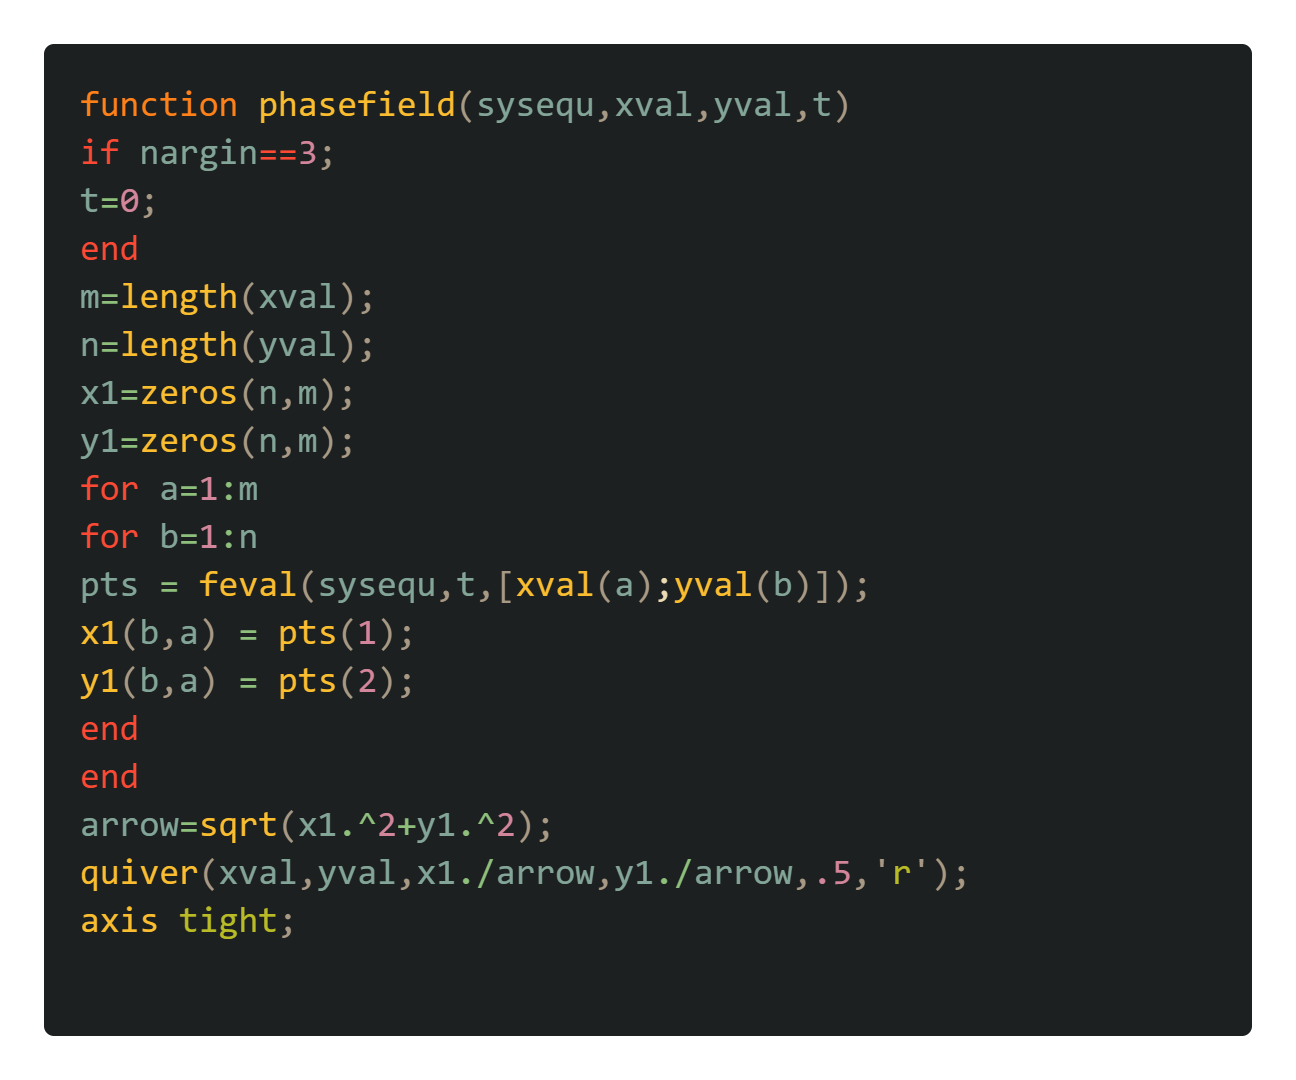
\includegraphics[scale=0.3]{PhasePortraitcode.png}\\
und habe dann im Command Window folgendes ausgeführt:
\subsection*{a)}
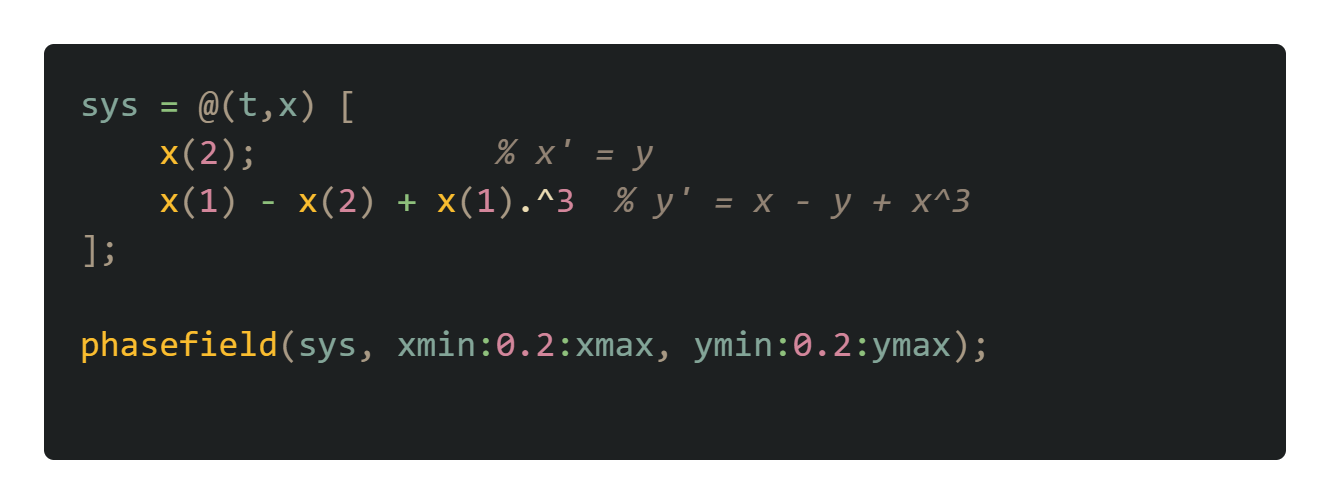
\includegraphics[scale=0.3]{aPhasefieldinit.png}\\
so erhält man:\\
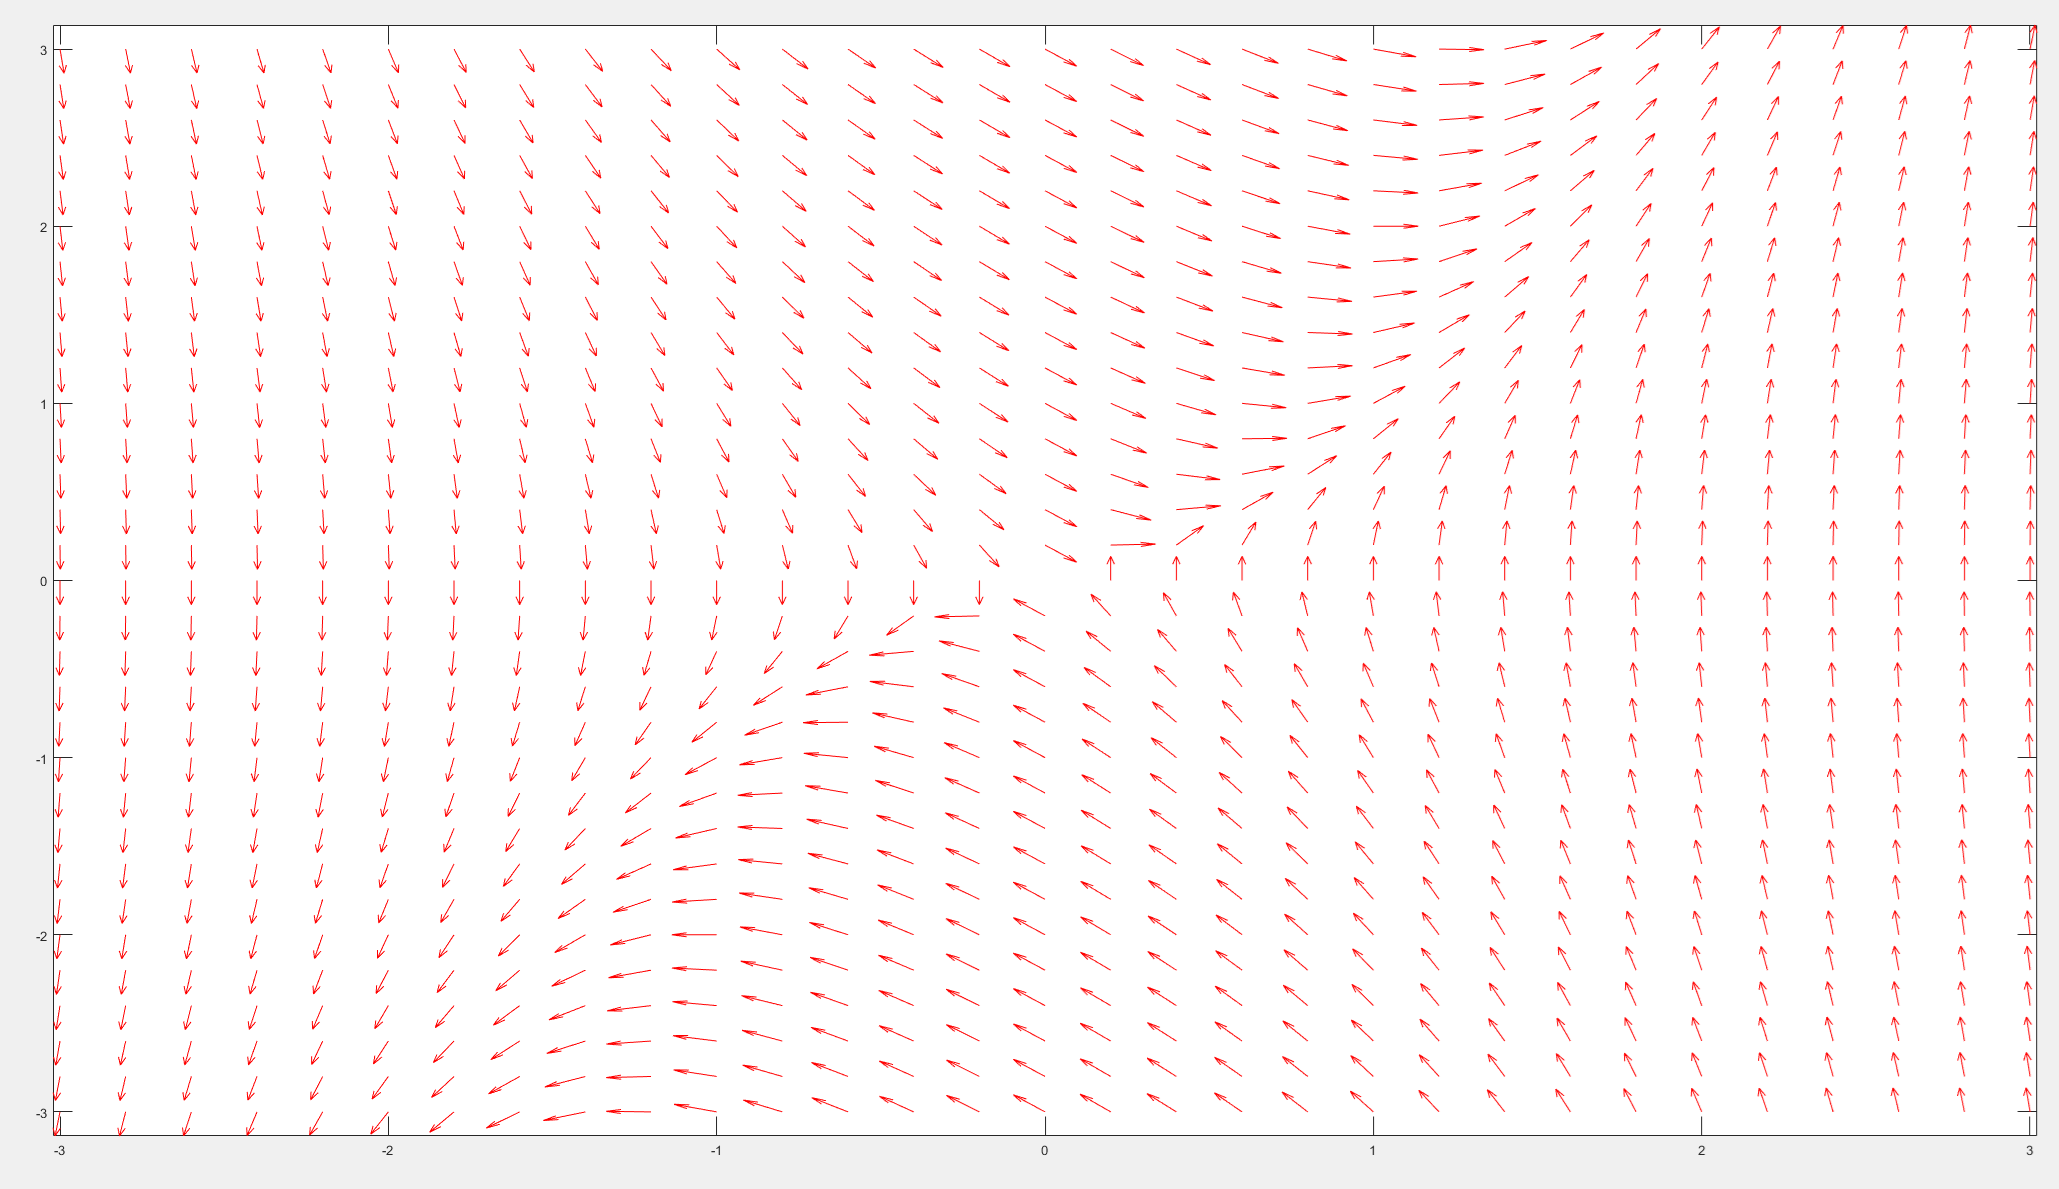
\includegraphics[scale=0.2]{aPhasefieldout.png}
\subsection*{b)}
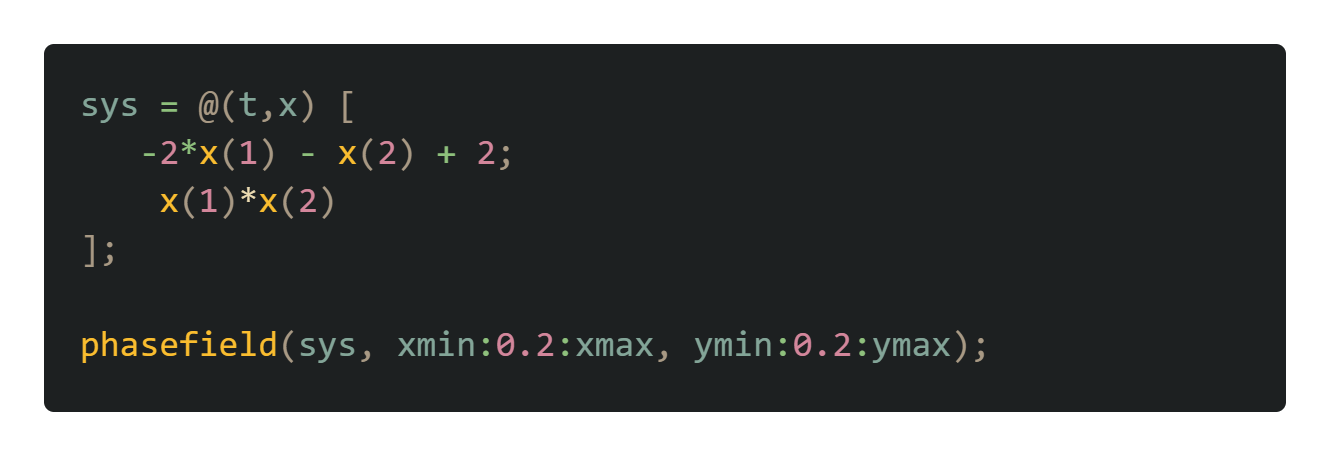
\includegraphics[scale=0.3]{bPhasefieldinit.png}\\
so erhält man:\\
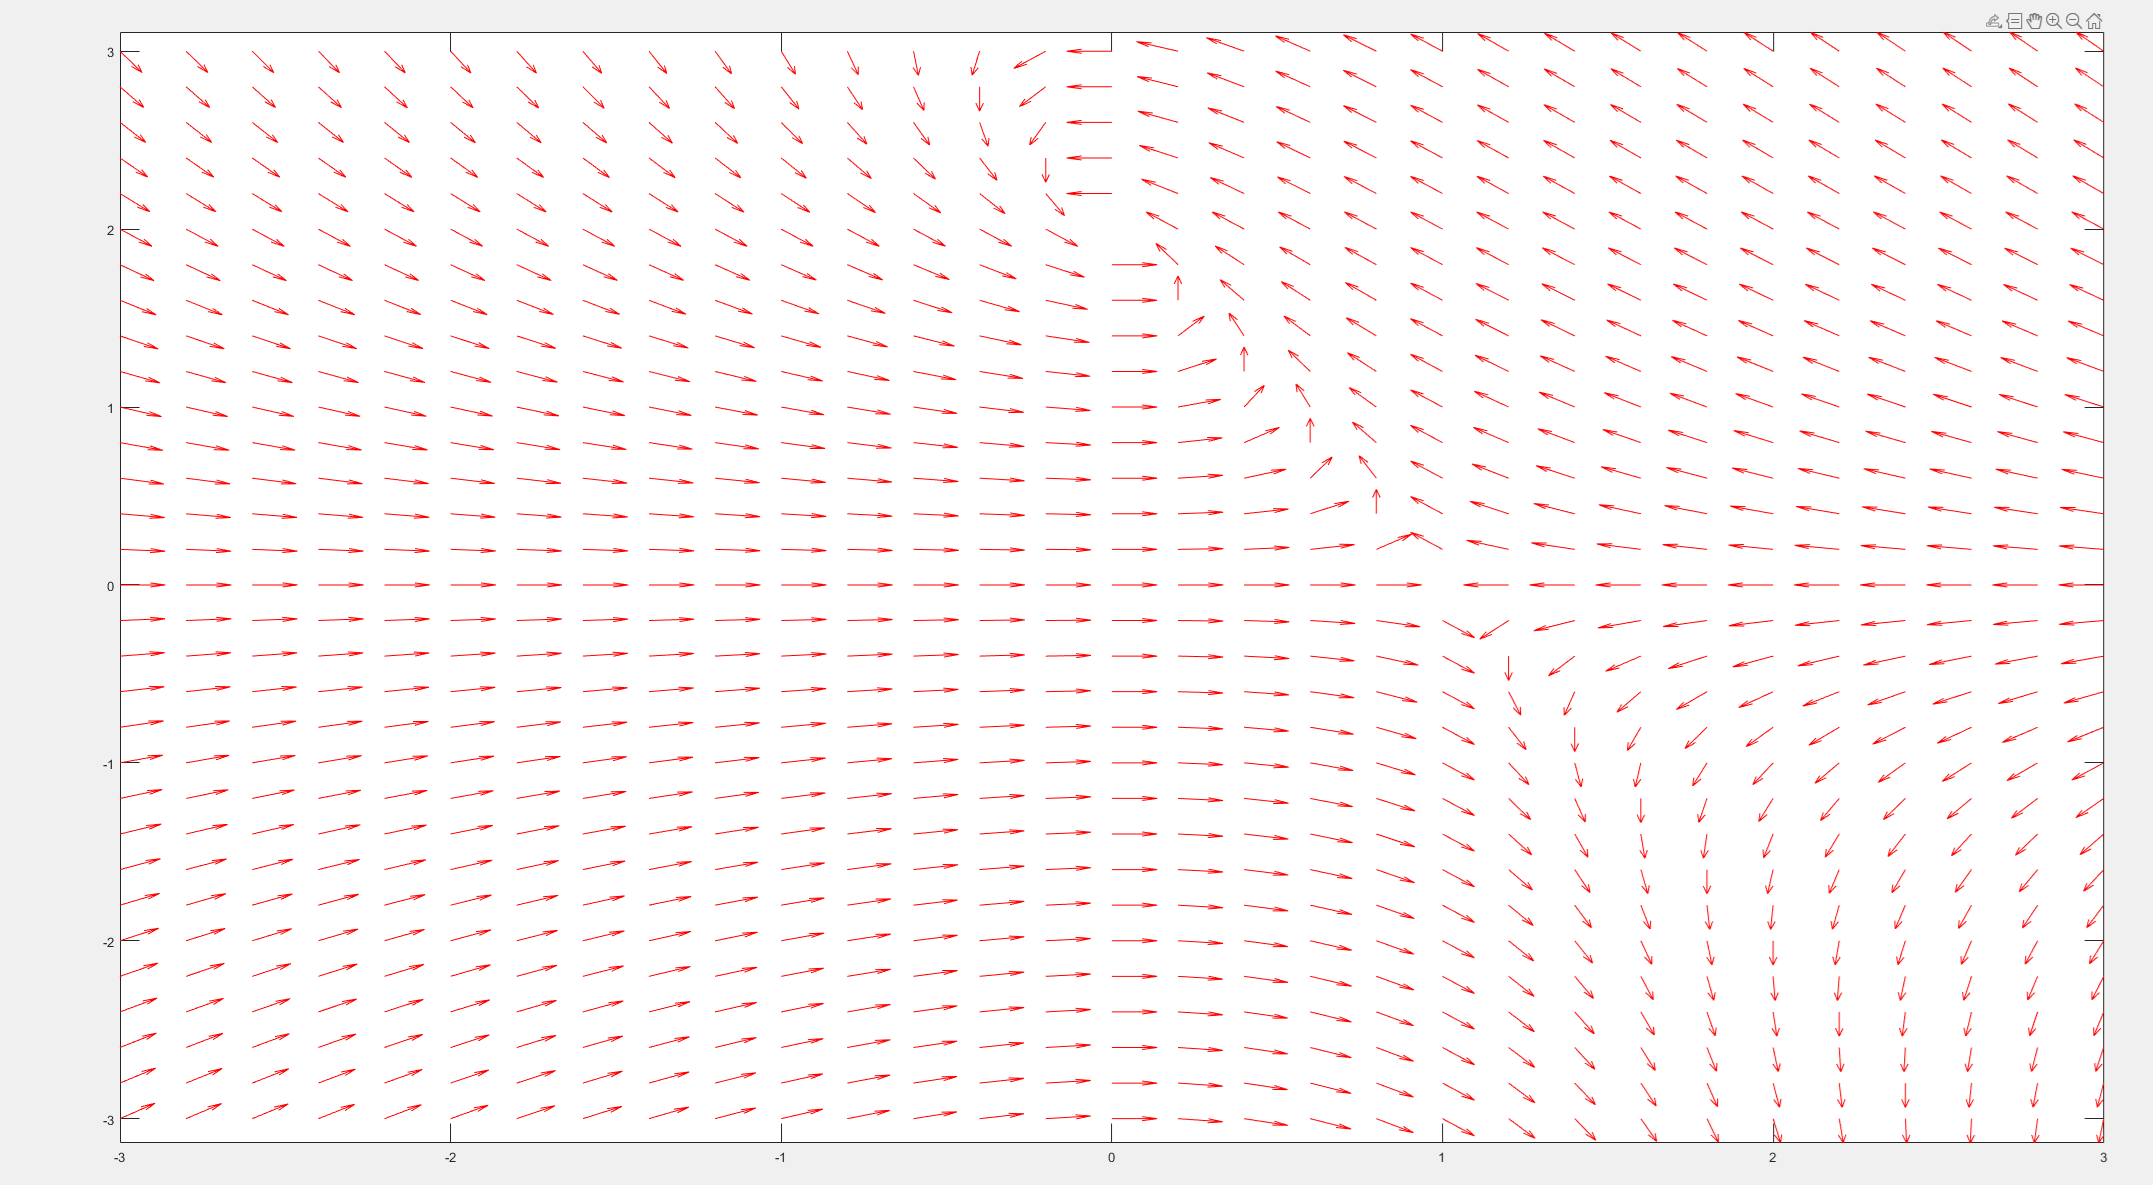
\includegraphics[scale=0.2]{bPhasefieldout.png}
\subsection*{c)}
$\mu$ ist natürlich variable ungleich 0 hier habe ich $\mu = -1$ gewählt.\\
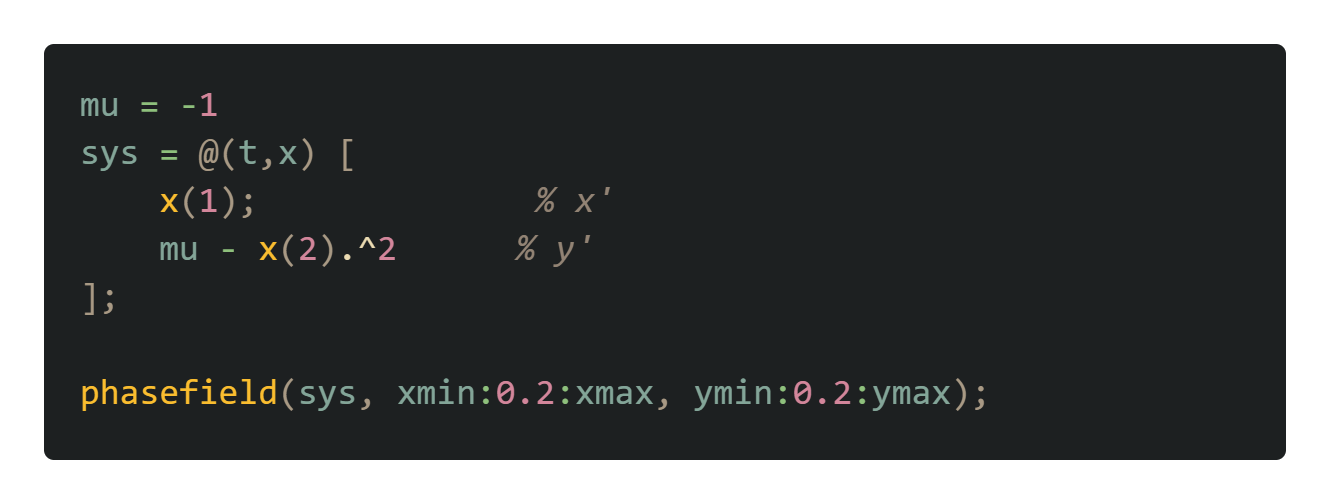
\includegraphics[scale=0.3]{muPhasefieldinit.png}\\
so erhält man:\\
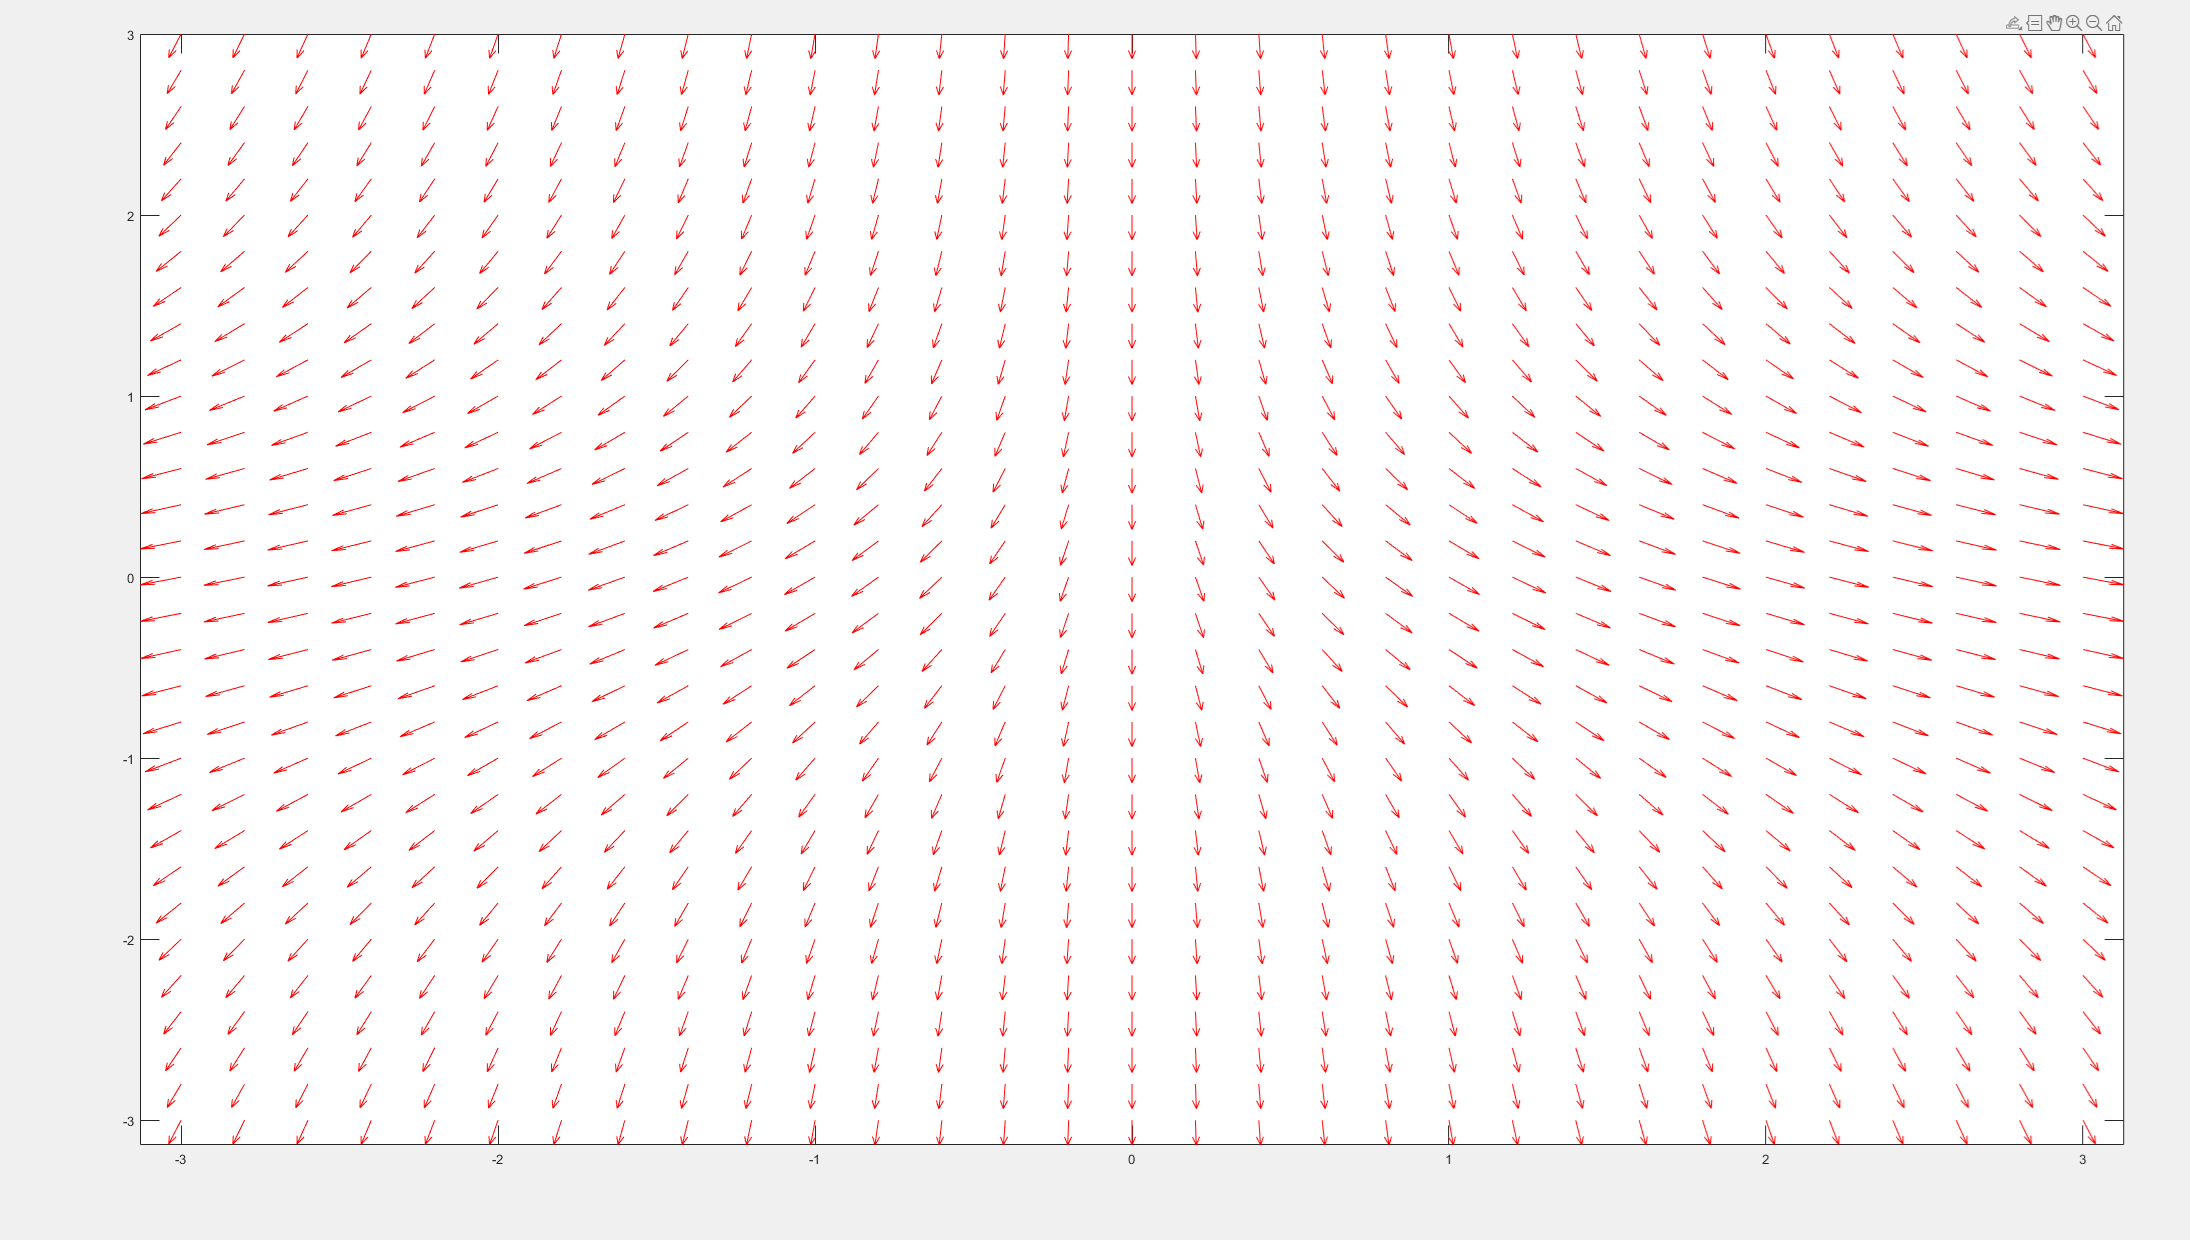
\includegraphics[scale=0.2]{muPhasefieldout.png}

\section*{Exercise 2. A simple Model for the Economy}
$I'=I-K\cdot S ,\quad S'=I-C\cdot S- G_0$ wurde gegeben.\\
\subsection*{a)}
C ist eine konstante die vor der Spending rate steht wenn C = 1 ist kann man diese dann aus der Gleichung raus schmeißen. Mithilfe einen Phasenportrait kann man die Verläufe der Funktionen I und S darstellen ausgehend von verschiedenen Startwerten, wenn man die Konstanten auf einen Wert setzt. Dann krigt man folgendes:\\
C=1\\
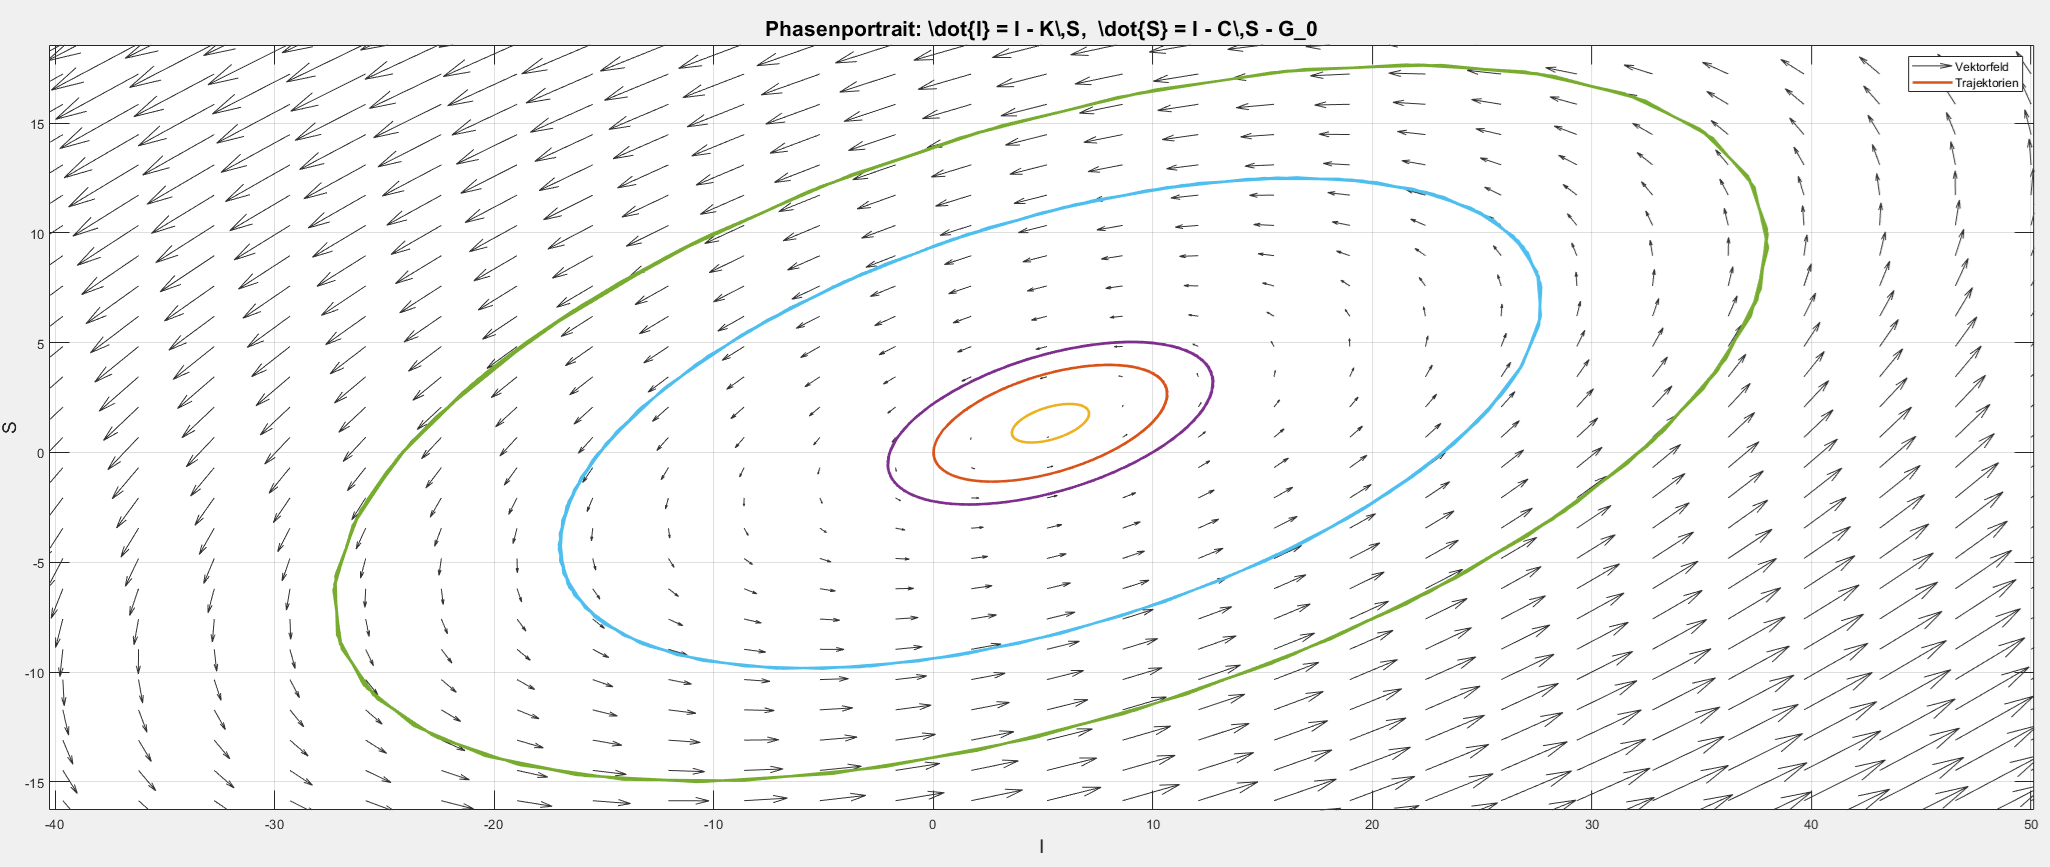
\includegraphics[scale=0.3]{PhasenportraitC1.png}\\
C=0.3\\
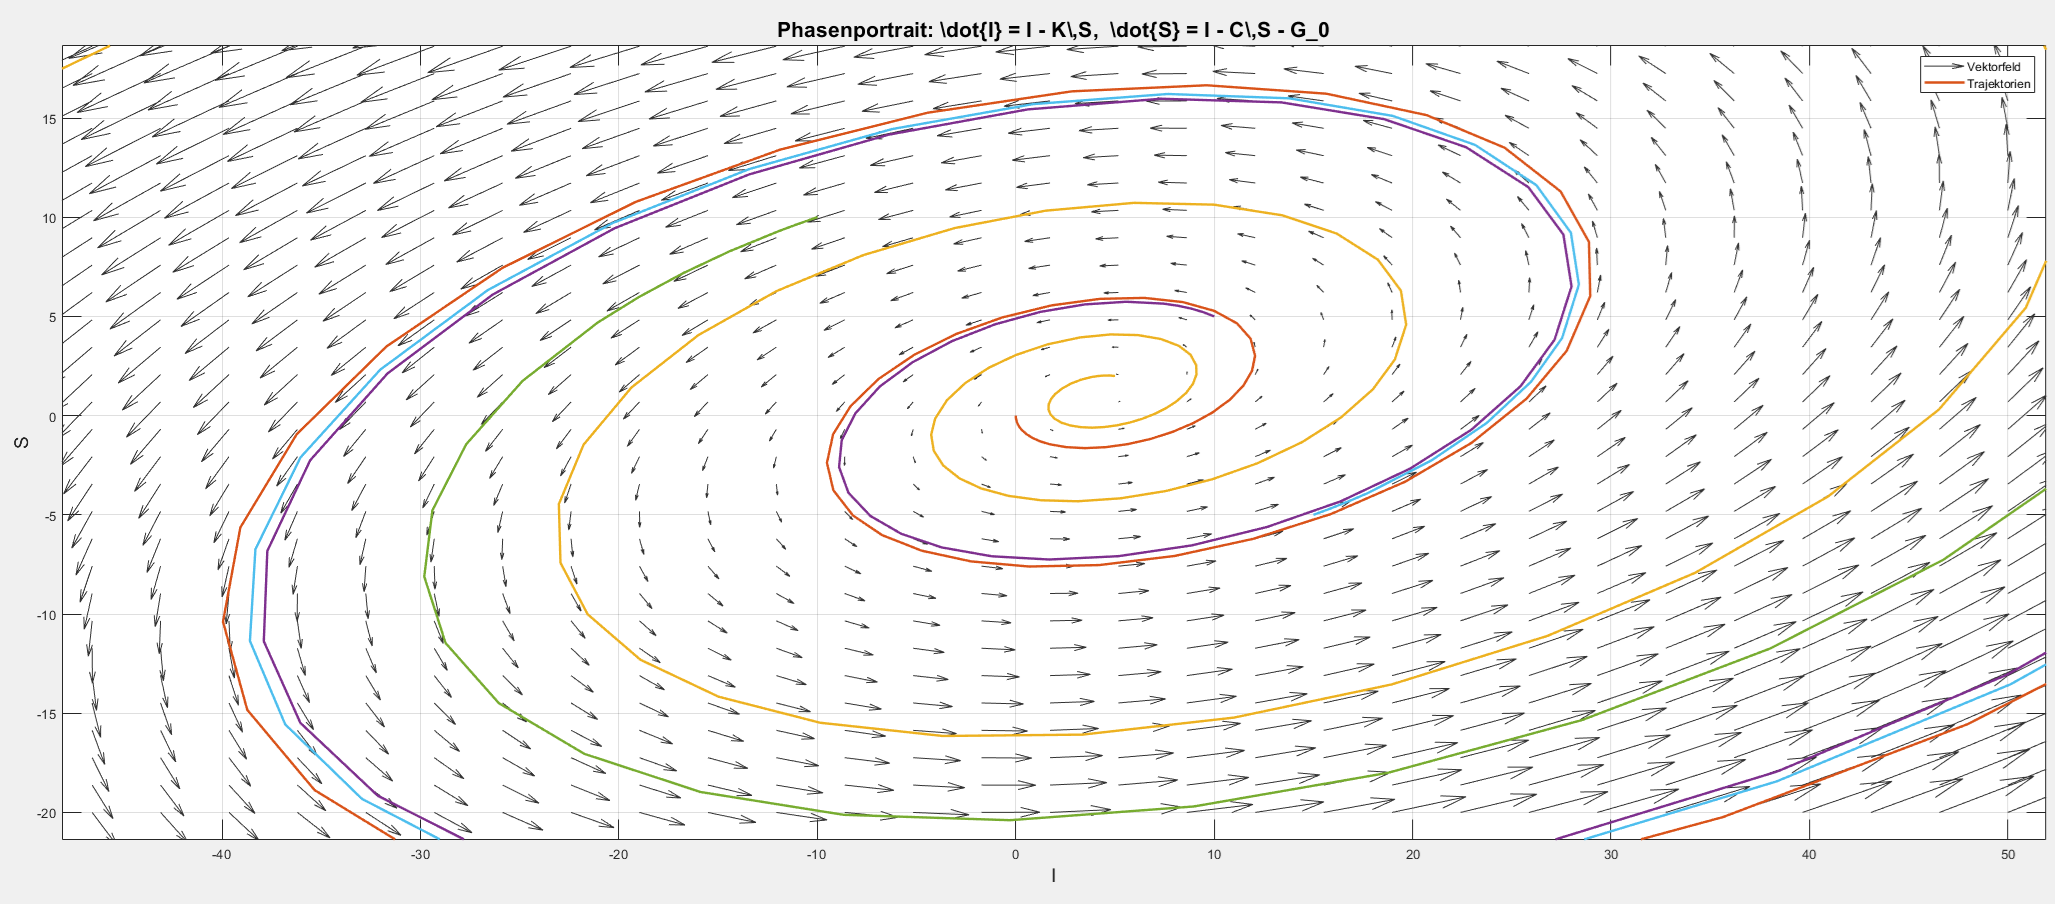
\includegraphics[scale=0.3]{PhasenportraitC04.png}\\
C=1.4\\
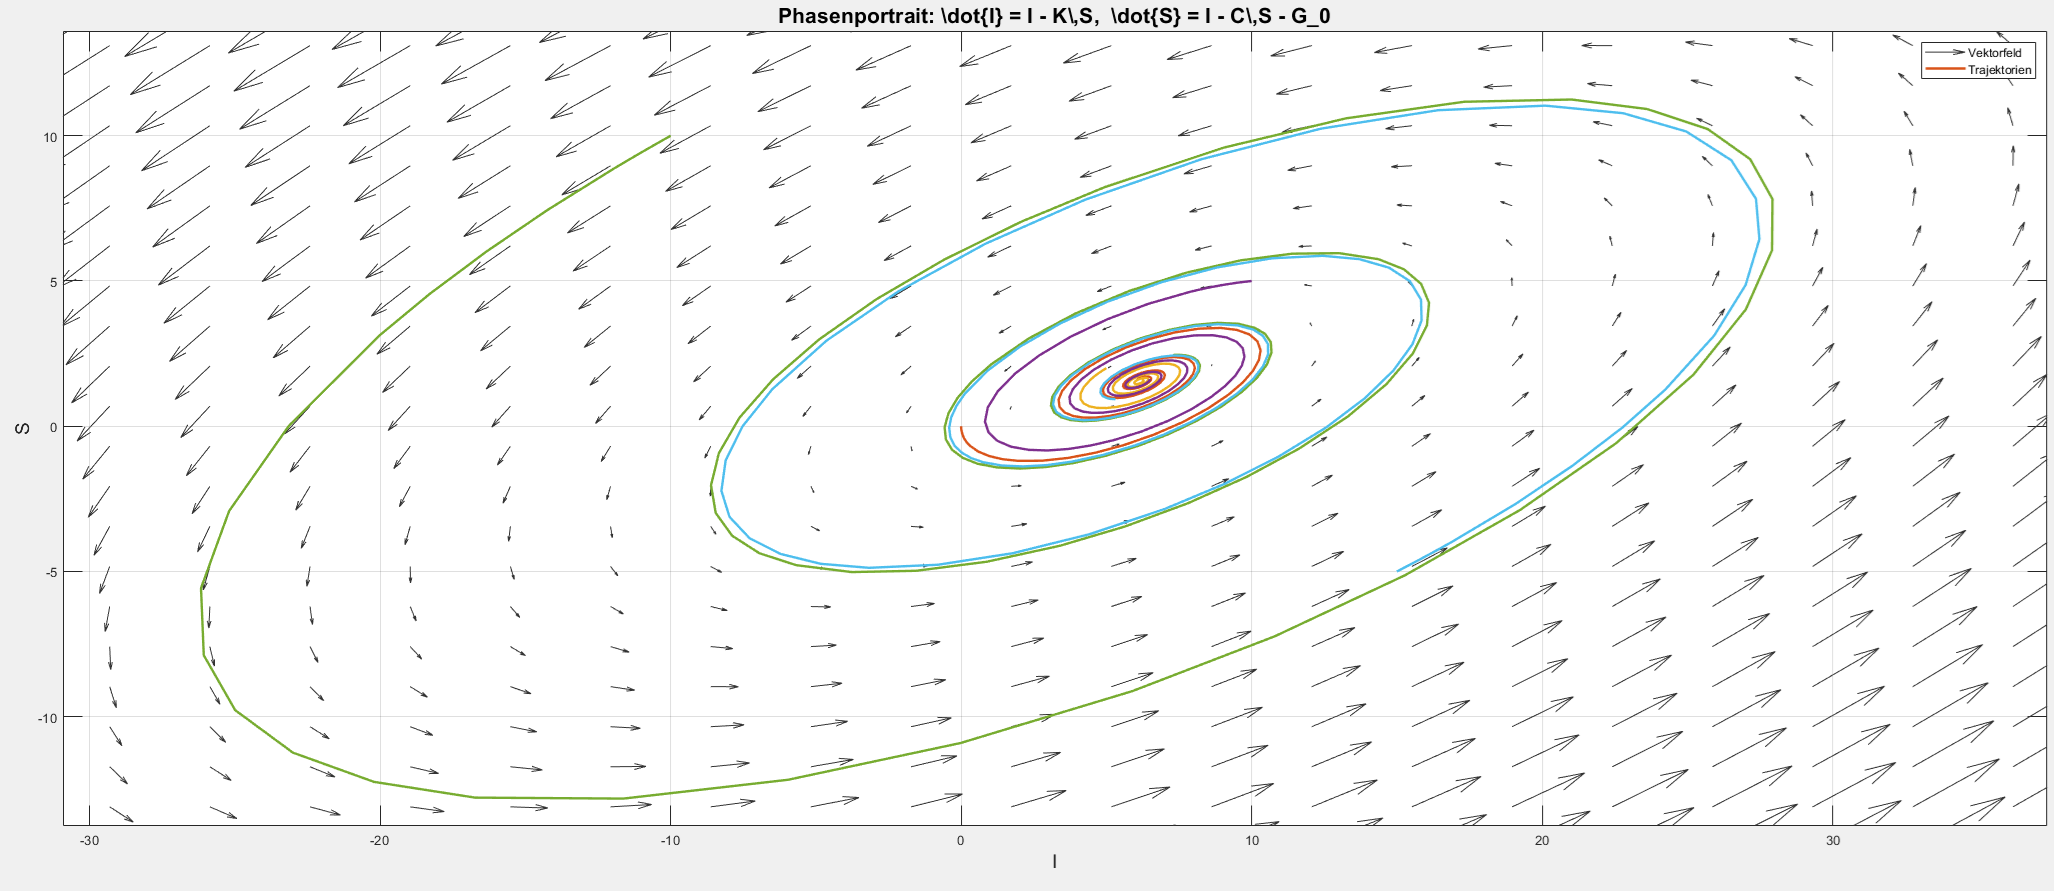
\includegraphics[scale=0.3]{PhasenportraitC2.png}

Wenn man C = 1 betrachtet sieht man das das System stabil kreist heißt man würde immer wieder die gleichen spending income dynamics haben. Bei C < 1 im gegensatz spiraled das system immer weiter nach außen heißt es gibt immer stärkere Schwankungen. Bei C > 1 nähert sich das system einen stabilen Punkt.\\
Code für die Phasenportraits:\\
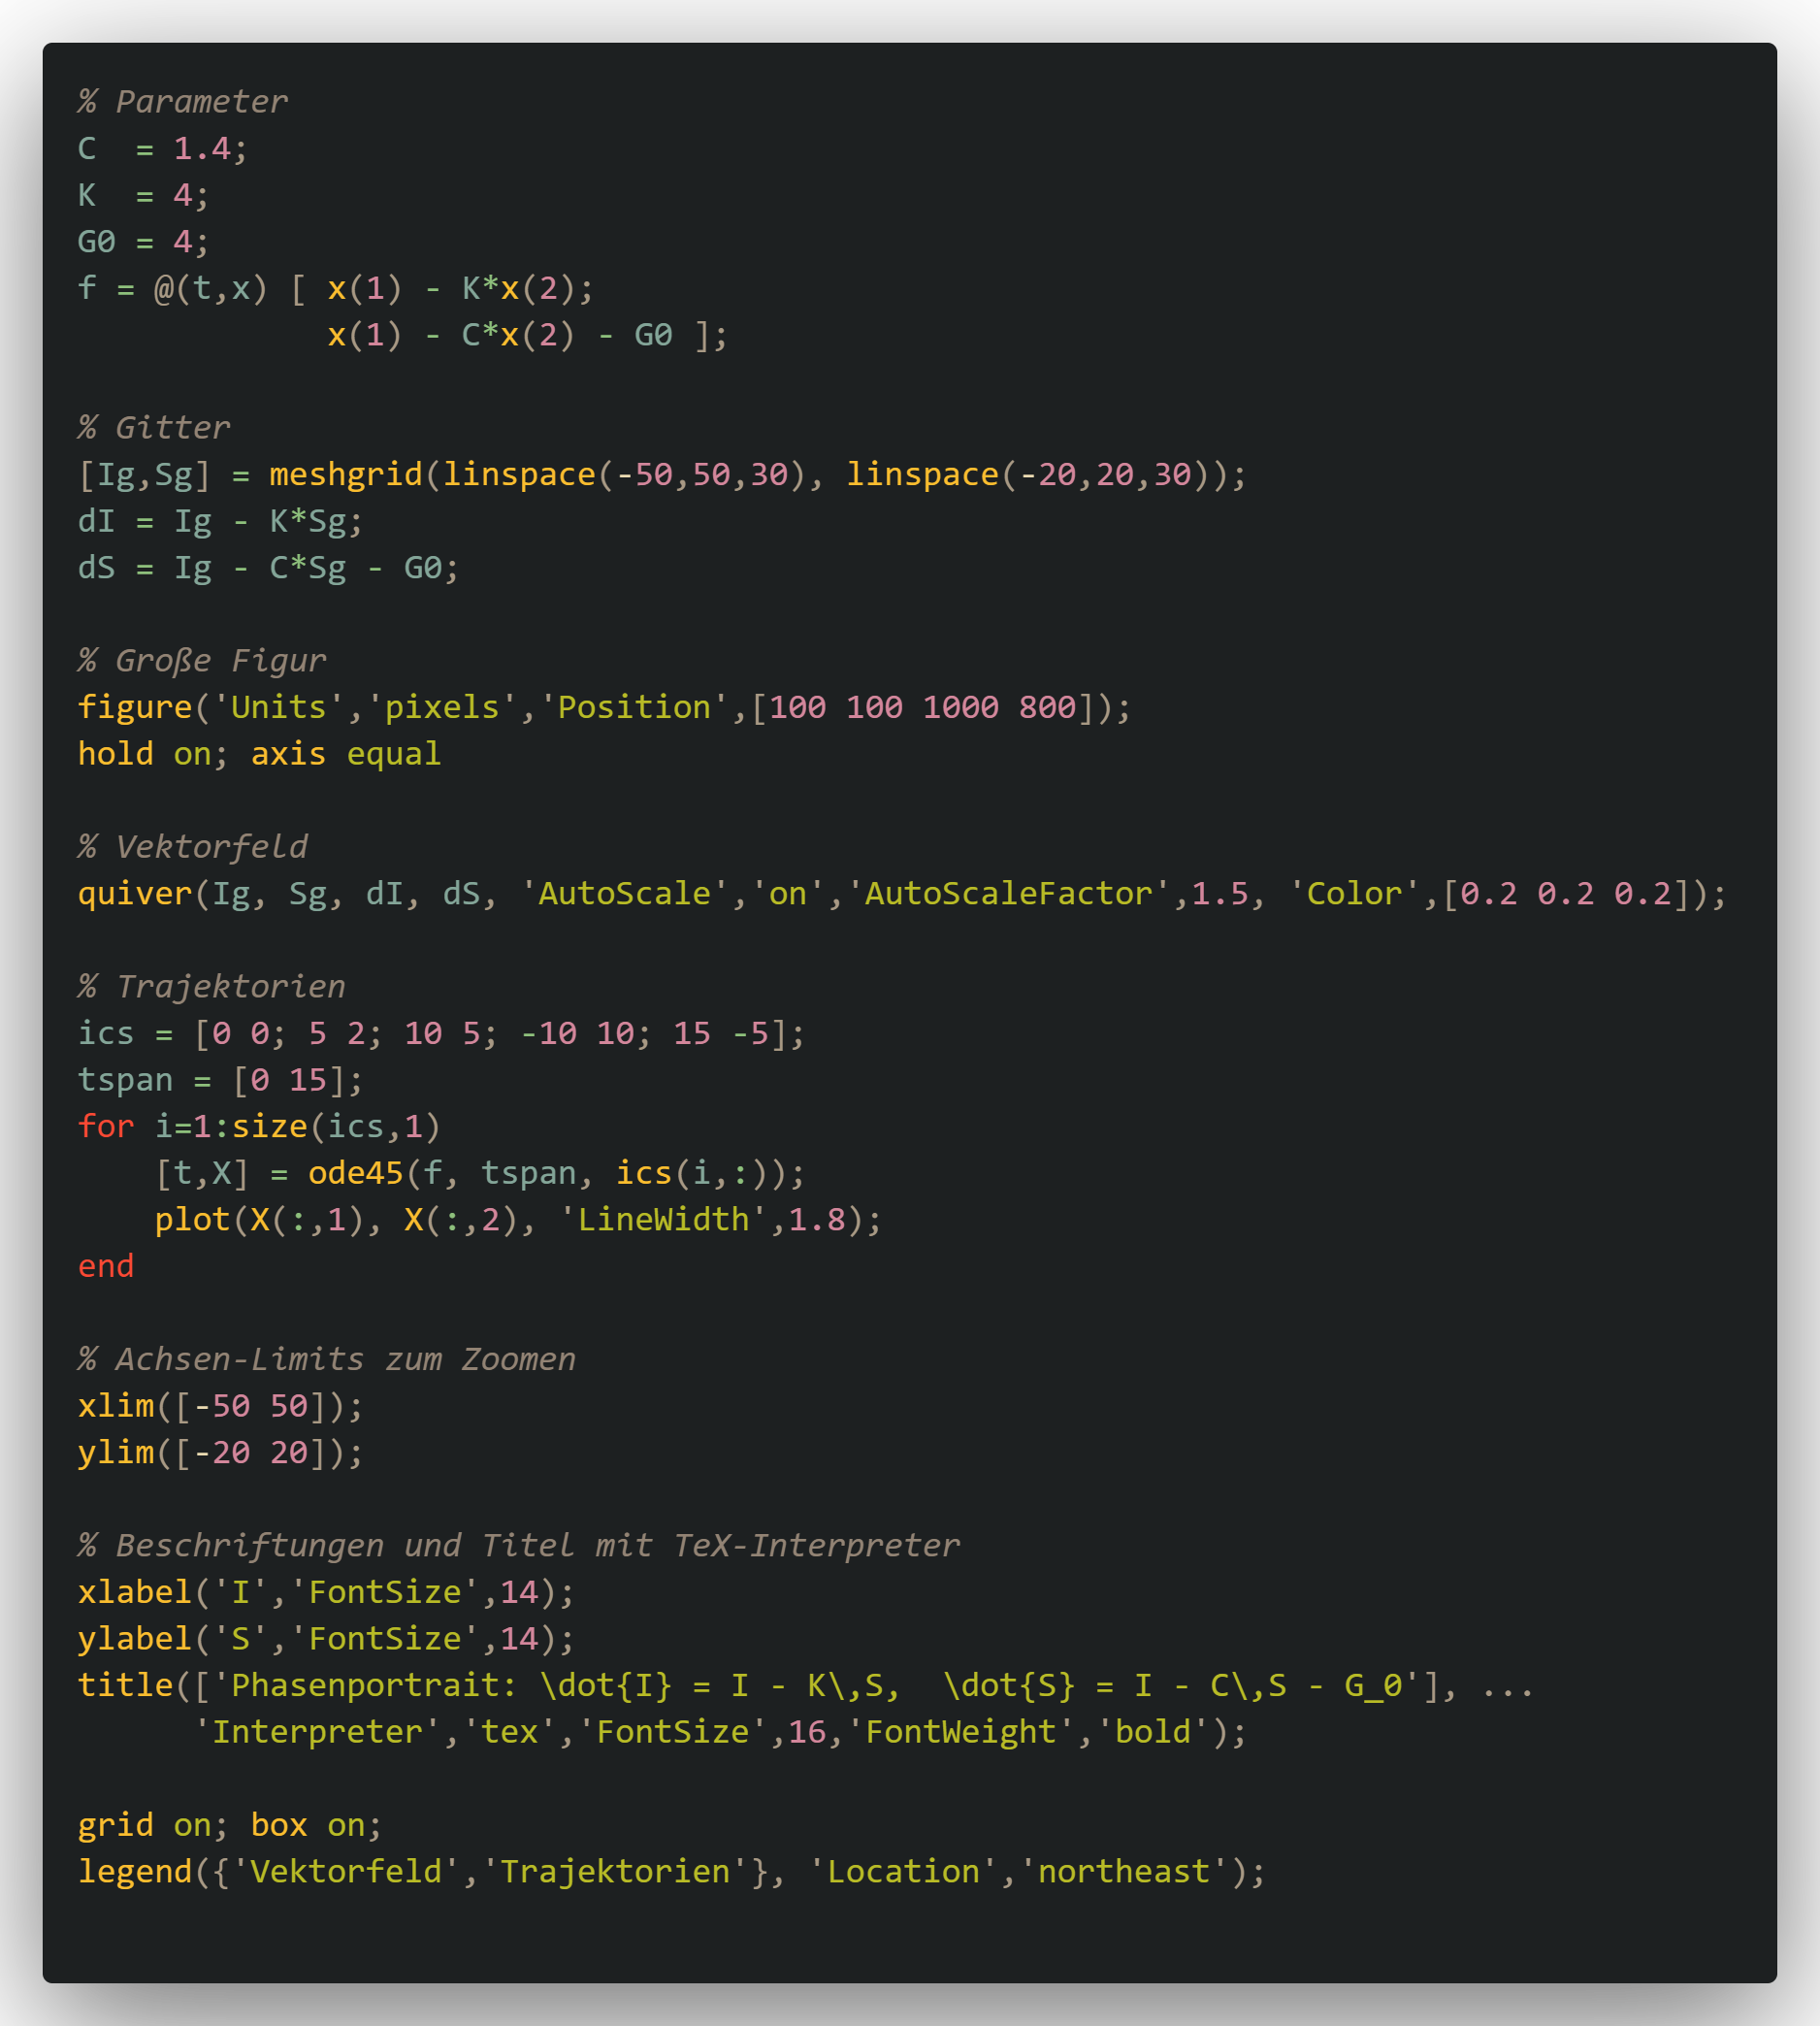
\includegraphics[scale =0.2]{code.png}
\section*{Exercise 3. }
Ich bin mir nicht komplett sicher was heir gefragt war. Ich habe das referenzierte SIR Modell nachgebaut:\\
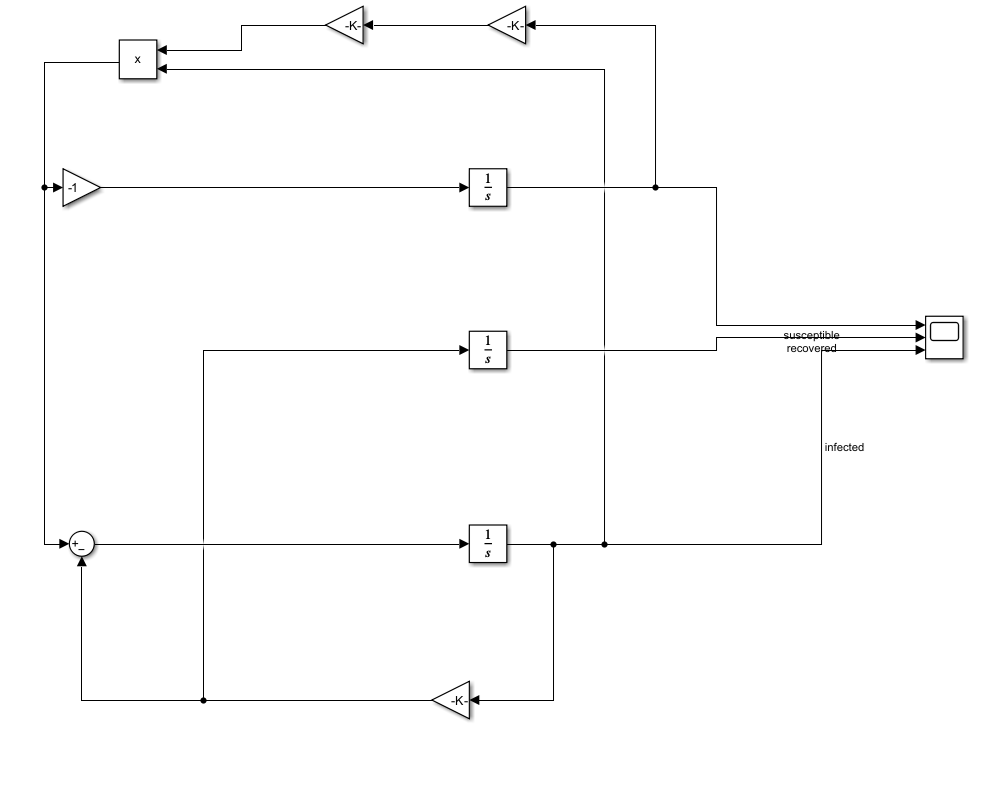
\includegraphics[scale=0.3]{sirModell.png}\\
Das Modell soll die Ausbreitung einer Krankheit simulieren. Im output kann man sehen, dass die Anzahl der infizierten Personen zuerst steigt und dann wieder sinkt. Gleichzeitig steigt die Anzahl der genesenen Personen.\\
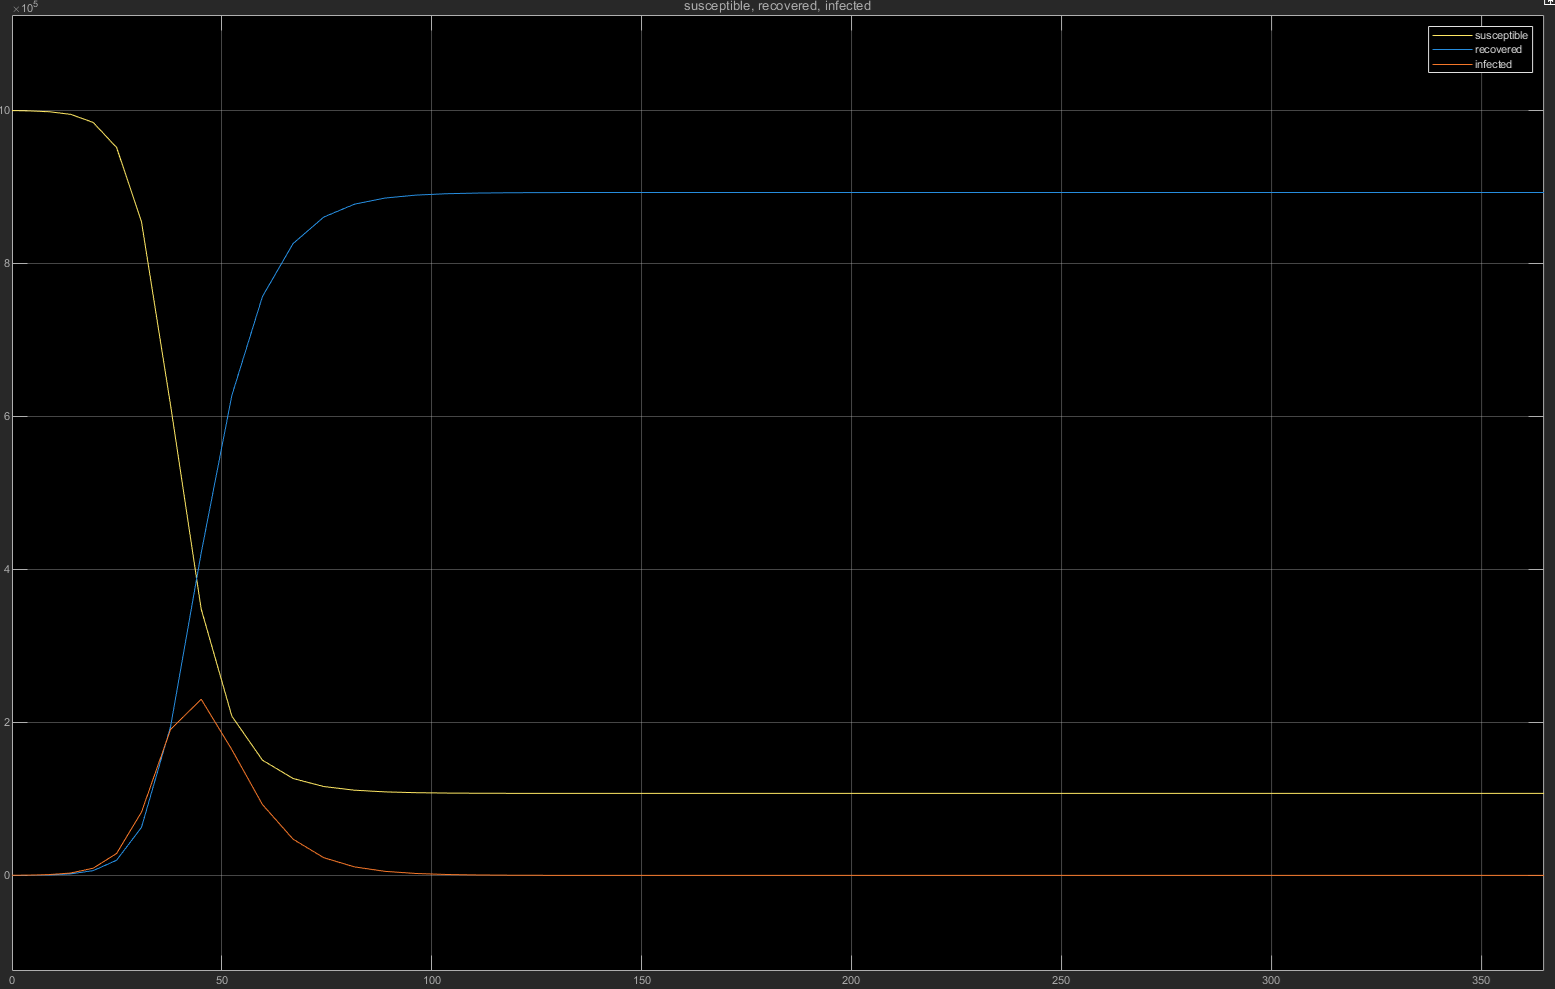
\includegraphics[scale=0.3]{sirout.png}


\section*{Exercise 4. Phase portraits of Van-der-Pol-System}
Ich habe das Modell aus der Aufgabe kopiert:\\
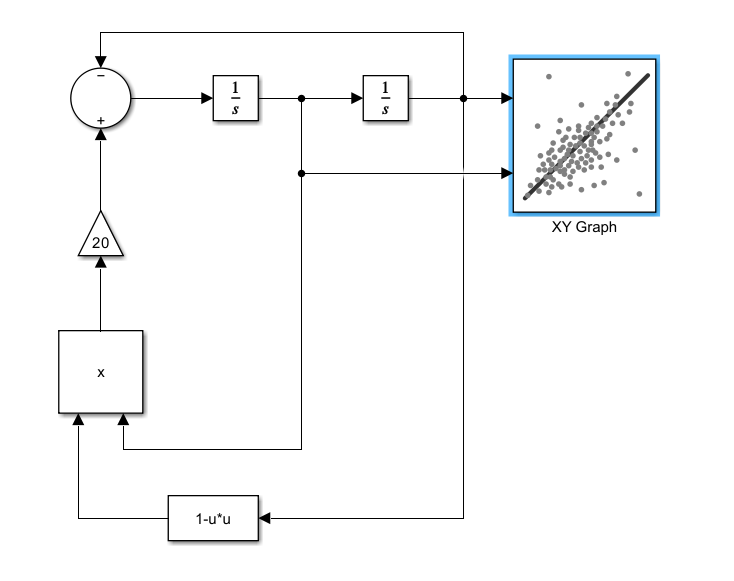
\includegraphics[scale=0.3]{E4.png}\\
und dann in der letzten gain die in der Aufgabe als $\mu$ gelabeld war die werte $0.1, 1, 5, 20$ eingesetzt. Das führt zu folgenden Graphen:\\
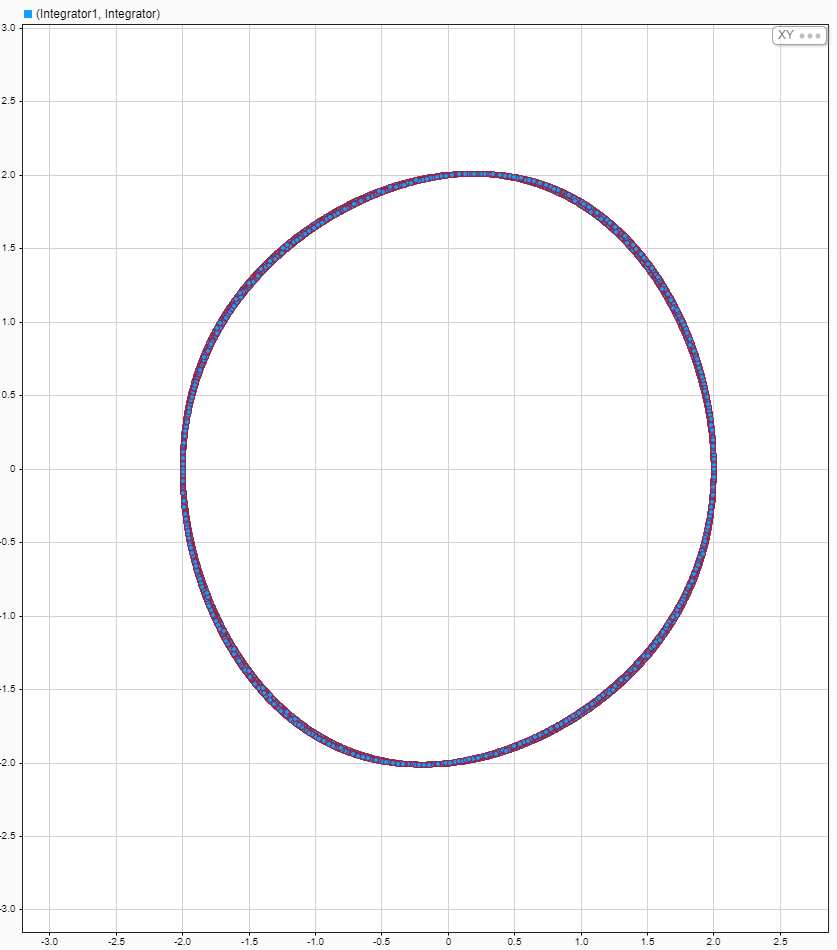
\includegraphics[scale=0.3]{E4mu01.png}
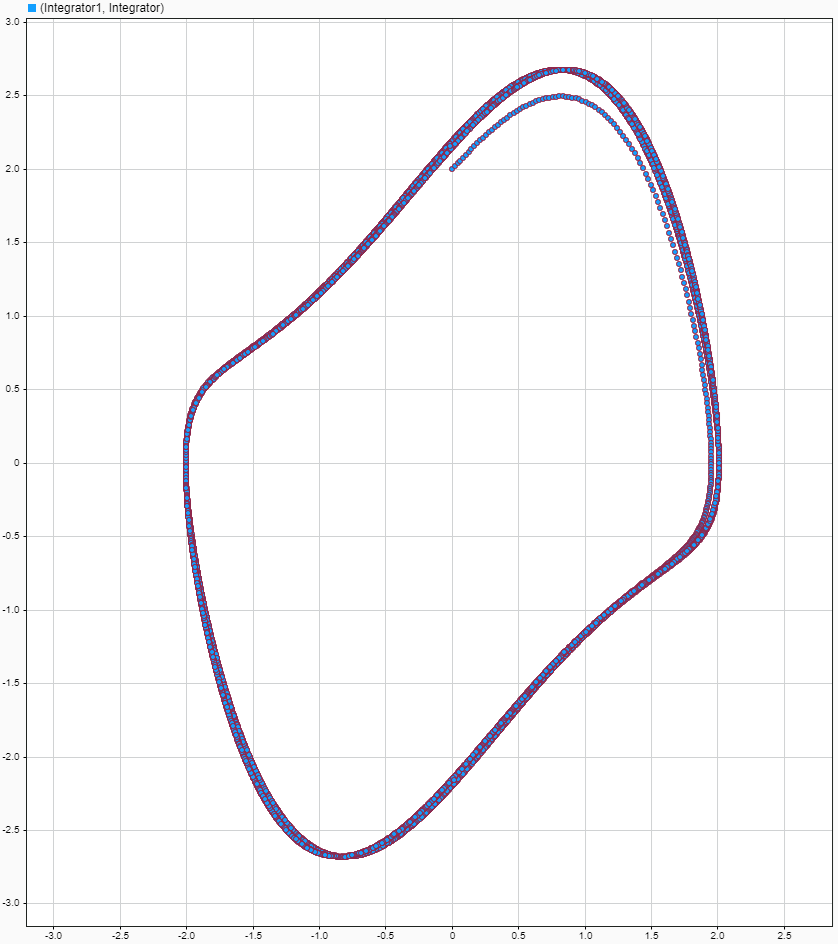
\includegraphics[scale=0.3]{E4mu1.png}\\
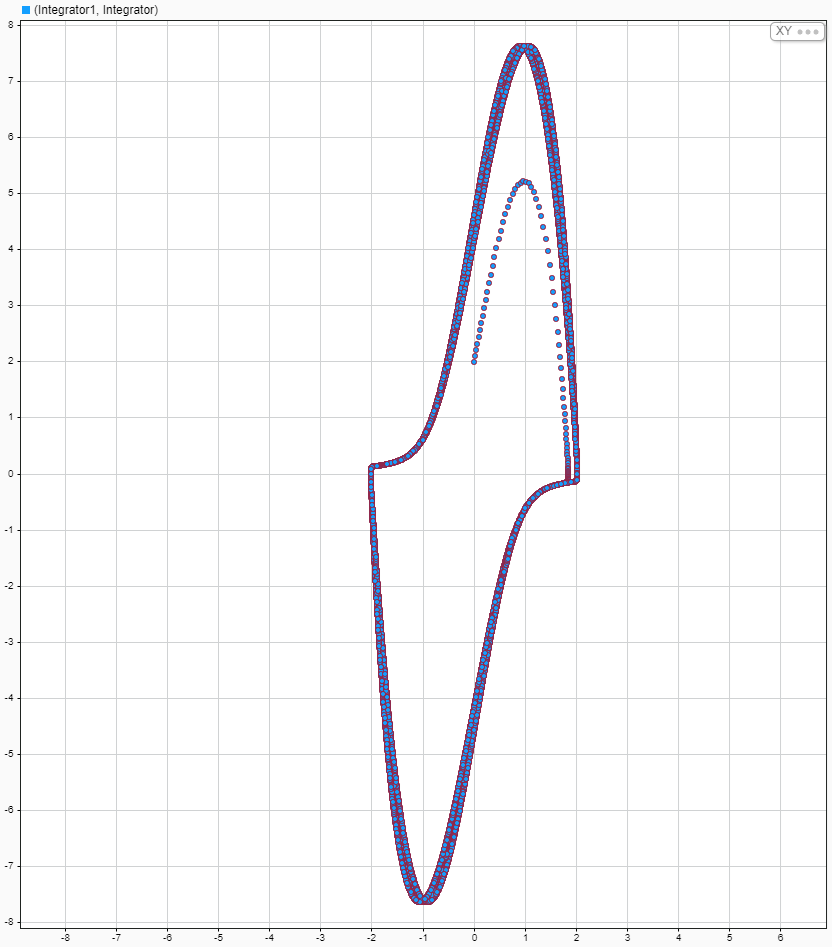
\includegraphics[scale=0.3]{E4mu5.png}
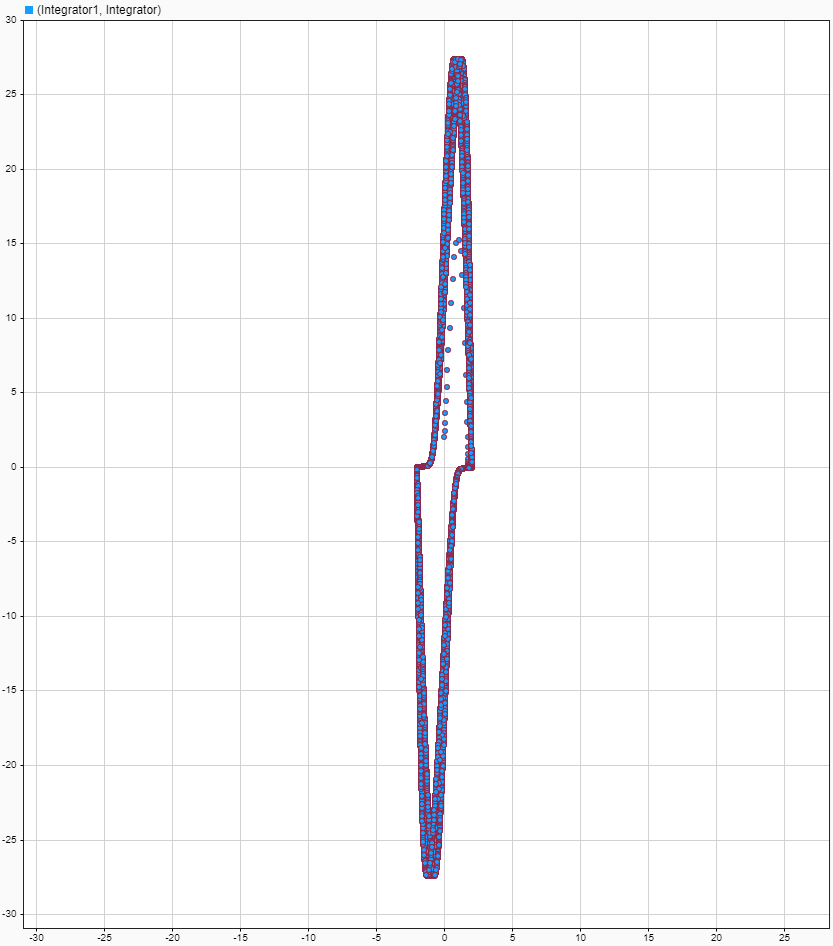
\includegraphics[scale=0.3]{E4mu20.png}\\

Dann habe ich die 'driving force' auf $0.5*\cos(t)$ gesetzt (ich habe $\omega = 1$ gesetzt). indem ich die Funktion im Funktionsblock geändert habe. Daraus erhält man dann folgende Graphen:\\
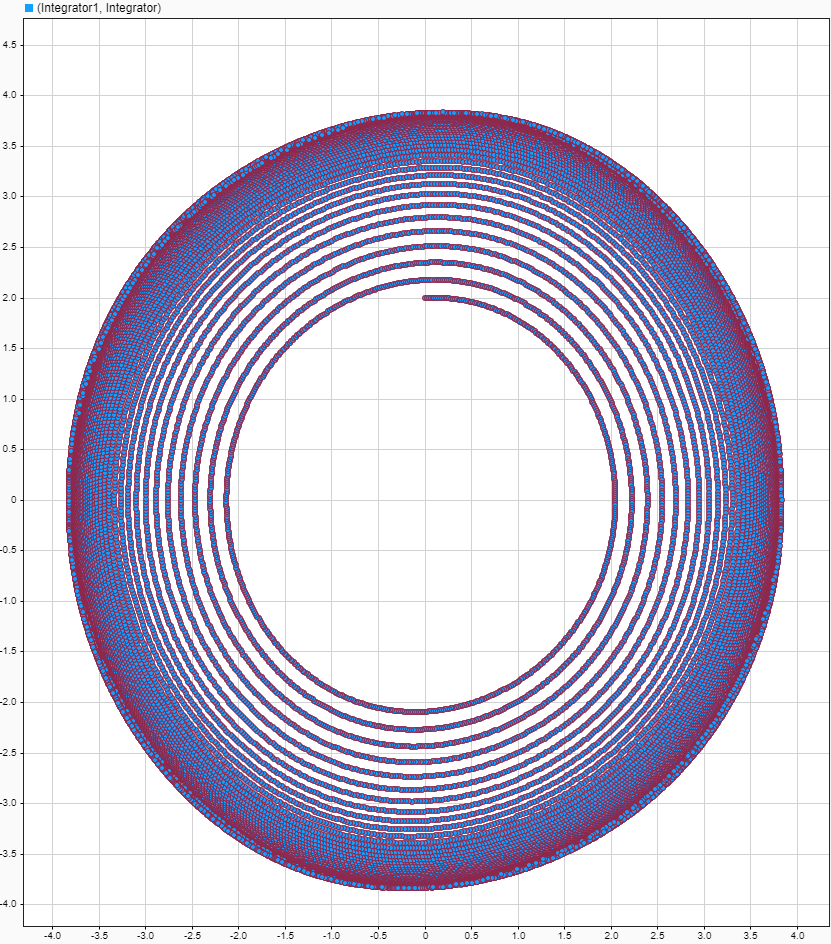
\includegraphics[scale=0.3]{E4mu01v2.png}
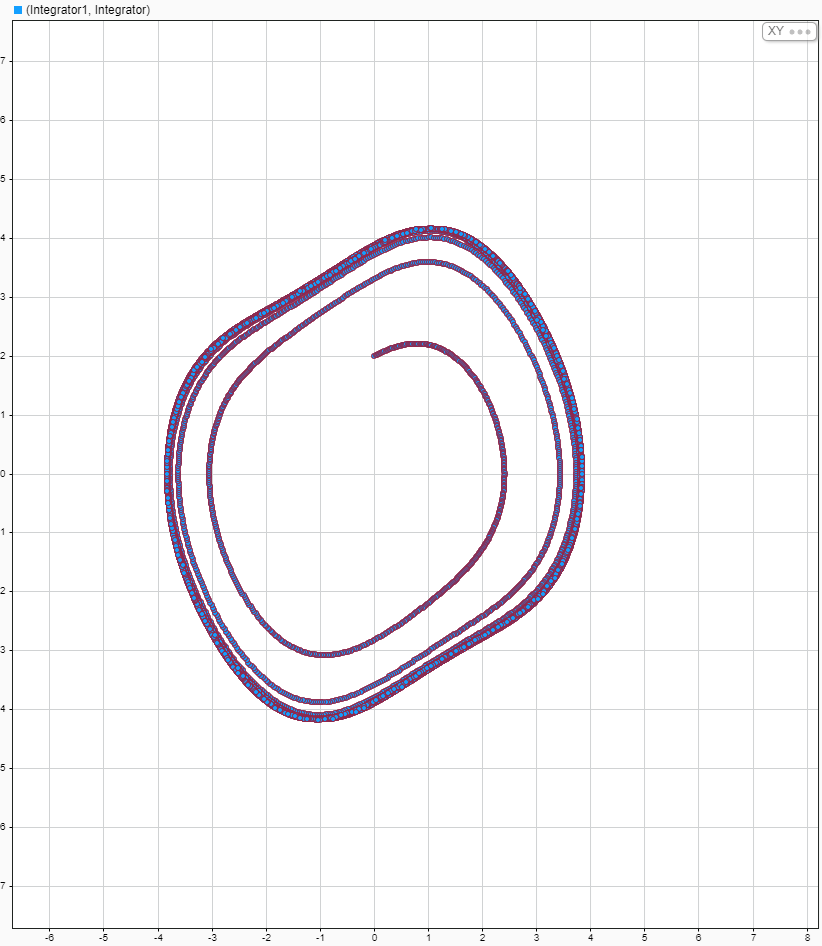
\includegraphics[scale=0.3]{E4mu1v2.png}\\
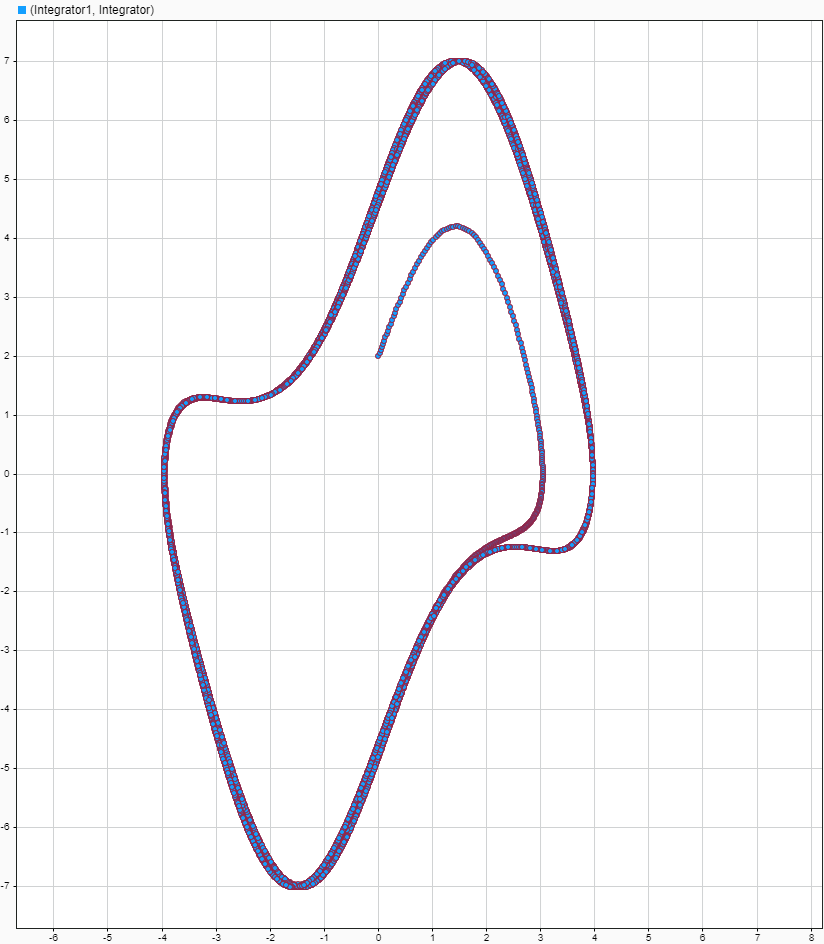
\includegraphics[scale=0.3]{E4mu5v2.png}
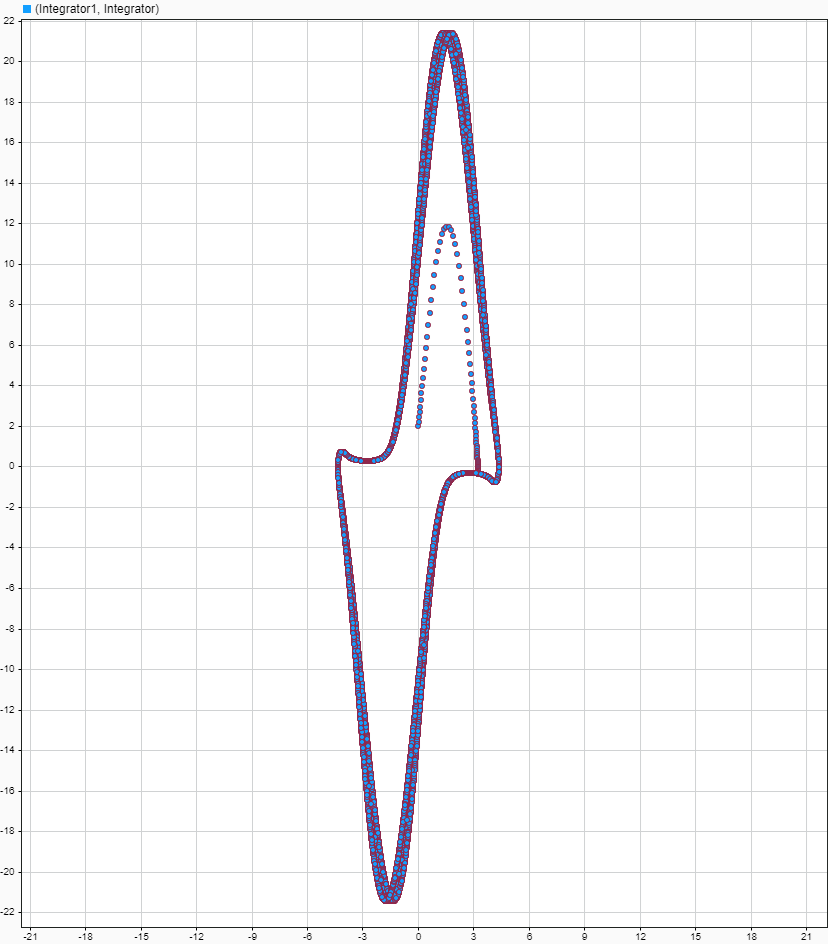
\includegraphics[scale=0.3]{E4mu20v2.png}\\
Man kann auf den neuen Graphen sehen, dass die veränderung der funktion dazu geführt hat das die Graphen mehr kreisförmig sind und und über die zeit weiter nach aussen wandern.\\

\section*{Exercise 5. Nonlinear pendulum driven by a periodic force}
Ich habe die Simulation aus der Aufgabe nachgebaut und dann die Parameter wie in der Aufgabe beschrieben eingestellt. Die verschiedenen ausgaben der Simulationen habe ich hier jetzt in der Reihenfolge der Aufgabe aufgelistet:\\
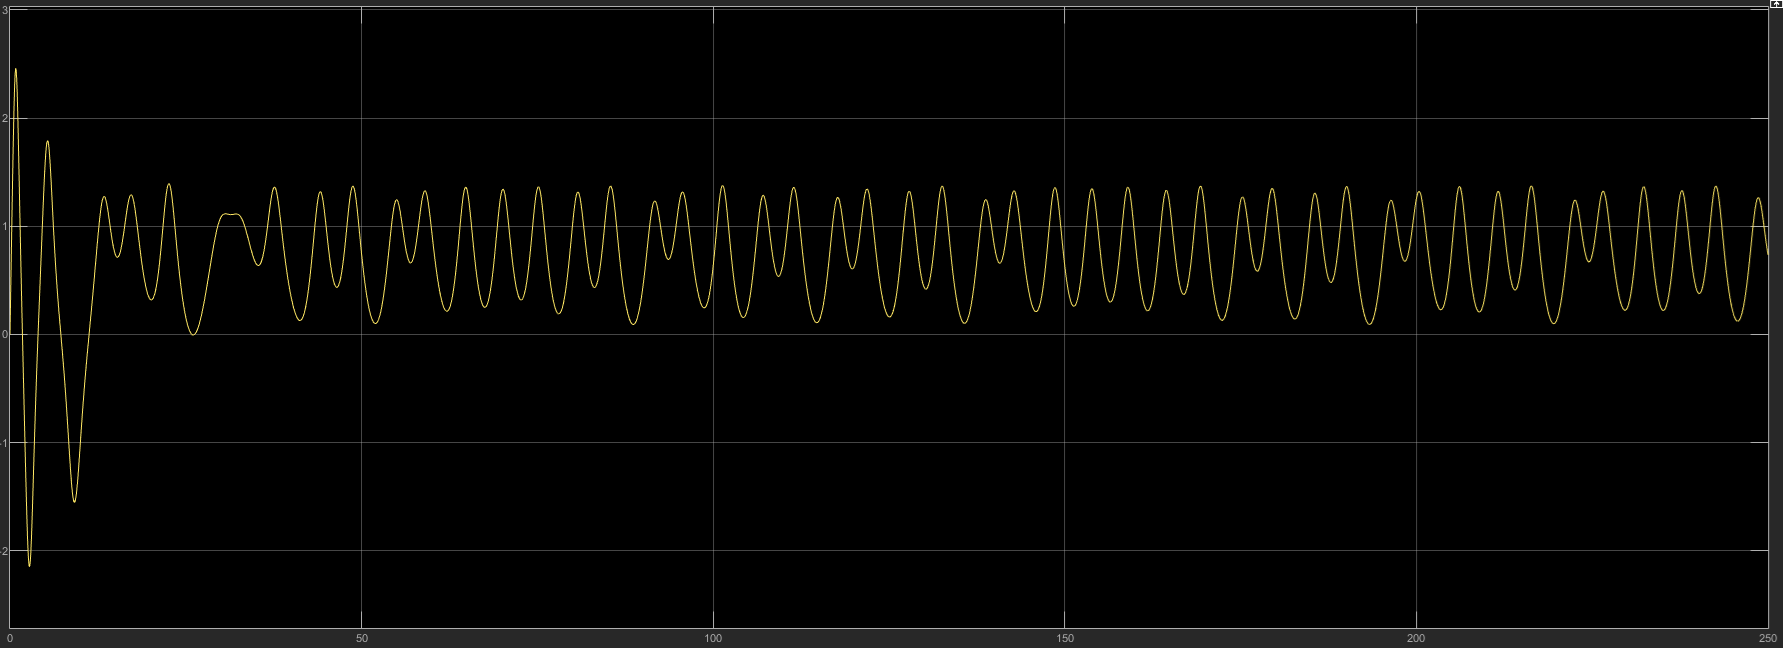
\includegraphics[scale=0.3]{nonlinv1.png}\\
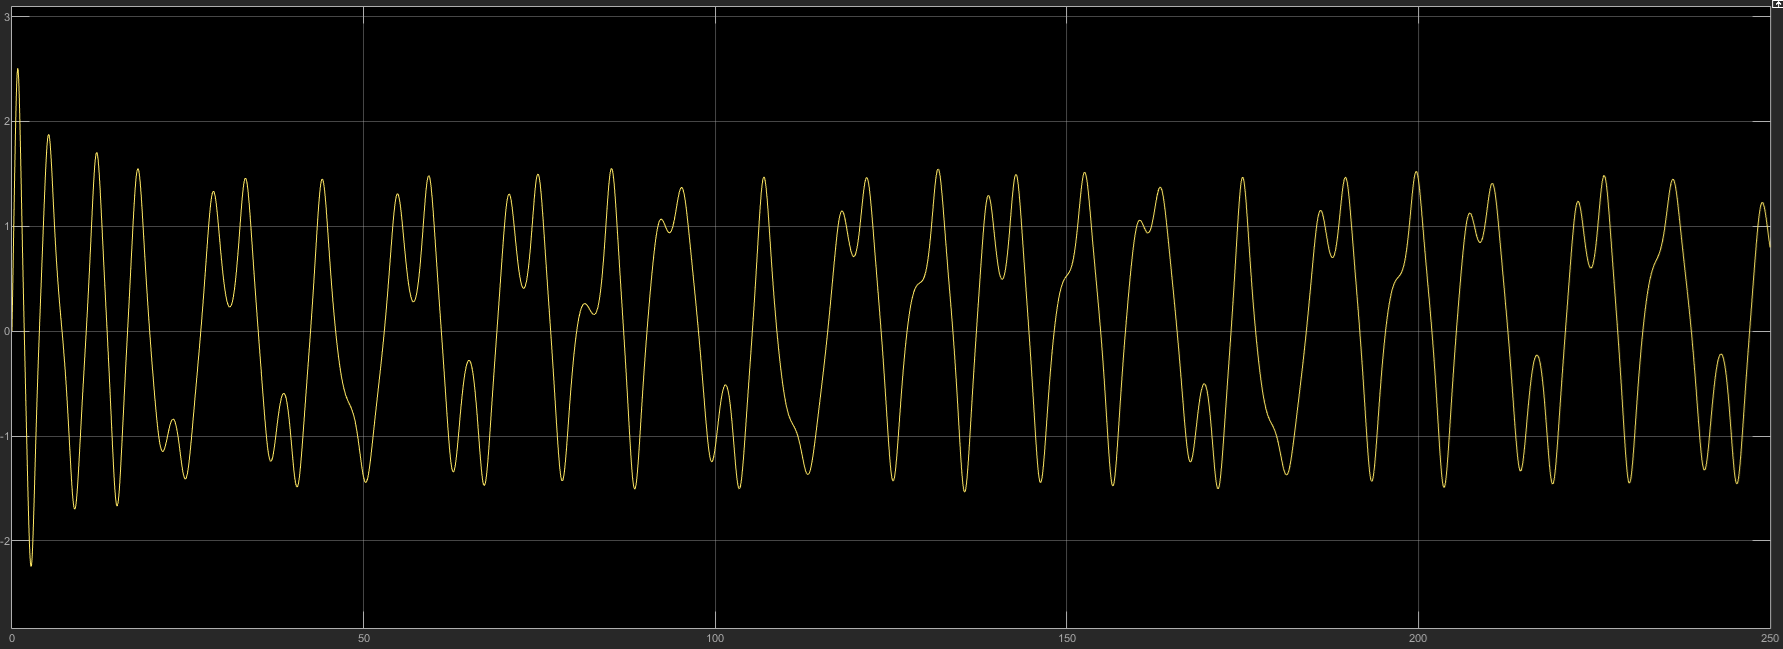
\includegraphics[scale=0.3]{nonlinv2.png}\\
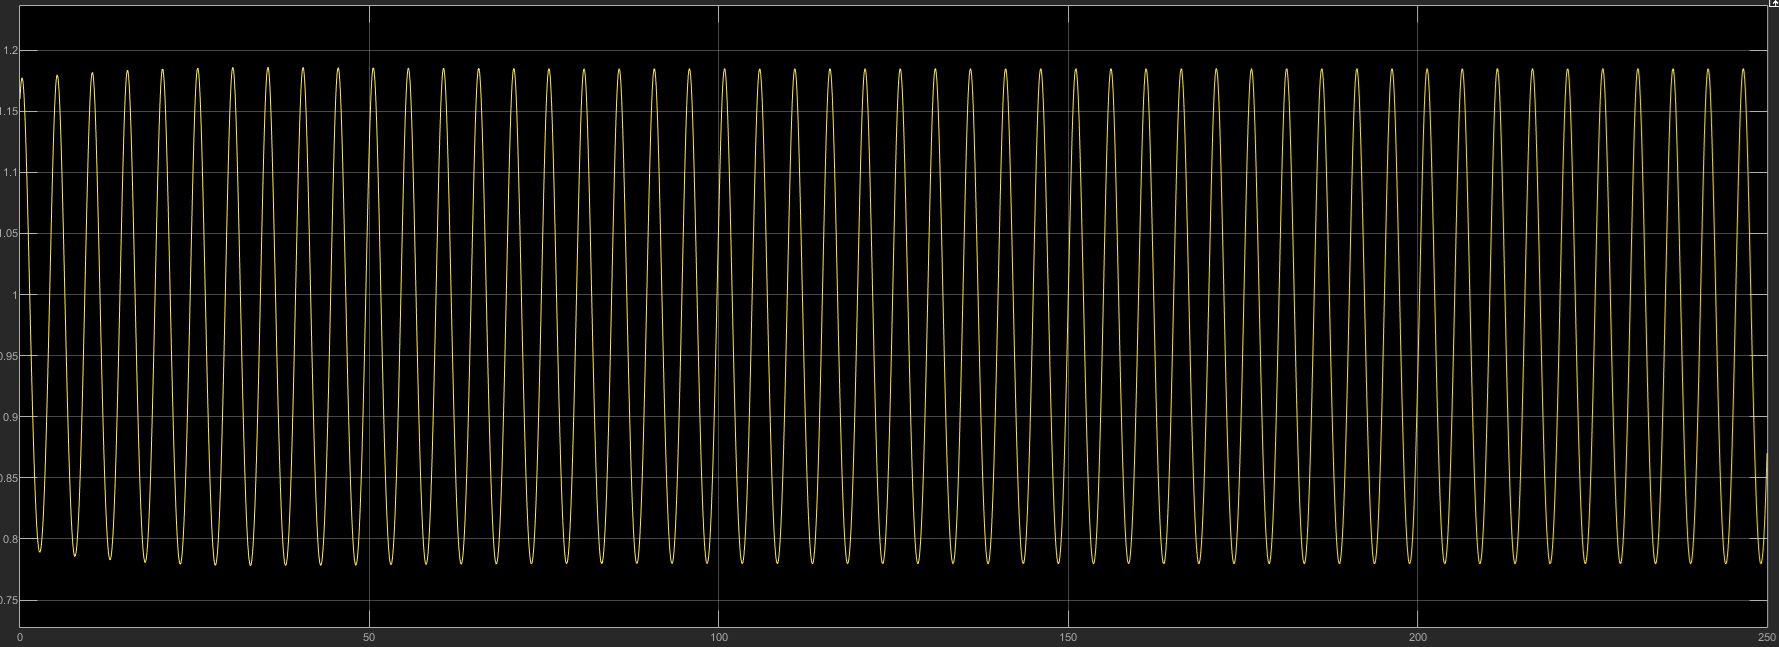
\includegraphics[scale=0.3]{nonlinv3.png}\\
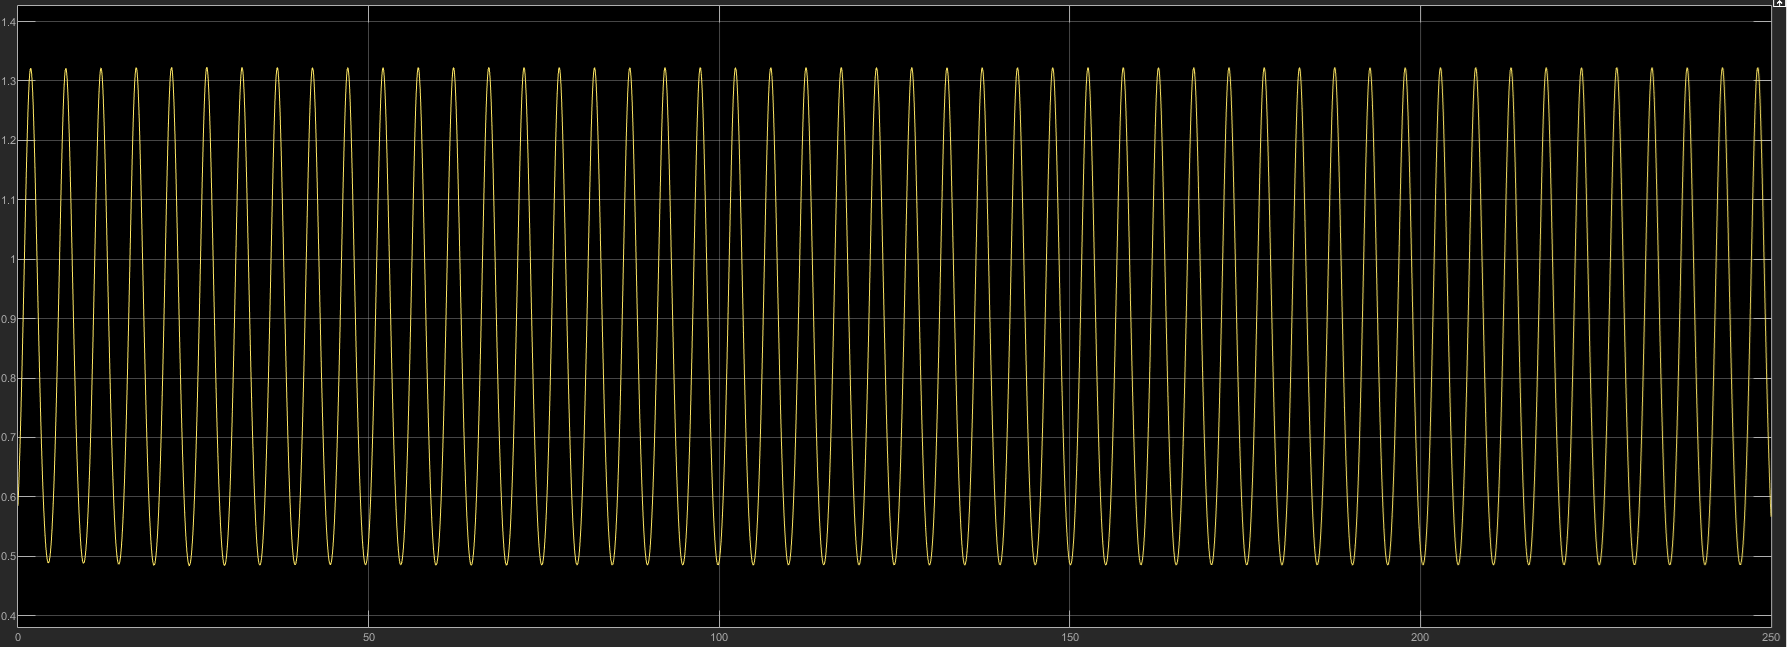
\includegraphics[scale=0.3]{nonlinv4.png}\\
Das System verhält sich in den ersten 50 schritten fast erratisch und dann stabilisiert es sich. Die Wellen danach ähneln klar sinus cosinus Verkettungen. Bei den letzten beiden ist die Frequenz der Schwingung aber im Vergleich zu den ersten beiden viel höher. Dies könnte an der extrem kleinen amplitude liegen.\\


\section*{\href{https://github.com/7hands/Angewandte-Modellierung-25-Colmant}{Github}}
Wie immer sind alle meine benutzten Dateien auf meinem Github zu finden.



\end{document}